\section{N2Sky Components}\label{N2Sky Components}

In the concept of N2Sky, lies a minimalistic and modern design. Dimmed tones of the UI components are used to make the end-user to feel like he is using a professional expert system. Every component and element was carefully thought out in order to keep the same atmosphere through the whole application. 

\subsection{N2Sky Frontend Application}\label{N2Sky Frontend Application}


Familiar elements and components help users to navigate easier through the application. It is important to have common components and elements and do not mix up together. Every component and every GUI element should have the self-describing purpose. Building user interface components and elements is almost the same as developing an UML diagram. It is possible to group common parts and maximize reusability \cite{mod_ui_book}. 

It is important to consider the multiple end-users, devices, platforms as well as environments that will be used. Through a heterogeneous context, only needed elements have to be displayed. It is necessary to make view prototypes to determine if the particular components are comfortable and easy to use \cite{Martinez2017}. 

\subsubsection{N2Sky Layouts Design}\label{N2Sky Layouts Design}


Design of N2Sky layouts was concentrated on principles of User interface design which were described in \cite{gui_layout}: 

\begin{description}
\item[Organise.]  All UI elements and components have to be ordered and not be chaotic. Randomise position or not understandable logic can confuse the user. 
\item[Consistency.] There are few types of consistency:
\begin{itemize}
\item Internal consistency, when elements are represented in the same place in familiar components. 
\item External consistency, when few elements are looking a little bit different, but with same functionality. This happens often on different devices, especially on mobile devices.
\item Real-world consistency, which brings real-world symbols into application UI elements.
\end{itemize}
\item[Screen Layout.] There are few screen layouts: 
\begin{itemize}
\item Grid layout, which organizes all components into blocks, like menus, navigation bars etc. 
\item Standardise the screen layout, which is mostly used on screens with restrictions.
\item Group related elements, which is usable for smaller screens.
\end{itemize}

In N2Sky Grid, the layout is used since it is easy to apply responsive design and reorganize grid items. 

\item[Navigability.] Navigation always needs to be on user focus or at least effortless to find. How it is supposed to work and where or how to use its elements have also an essential importance.
\item[Economize.] Following rules have to be applied: 
\begin{itemize}
\item Simplicity
\item Clarity
\item Distinctiveness
\item Emphasis
\end{itemize}
\item[Communicate]. The layout has to apply accuracy, typography, symbolism, multiple views to help the user communicate with the application.
\end{description}

\subsubsection{N2Sky Fundamental Layout}\label{N2Sky Fundamental Layout}

The N2Sky Fundamental Layout is represented by basic styling of the N2Sky application as is shown in figure \ref{fig:layout_basic}. 

\begin{figure}[H]
\begin{center}
  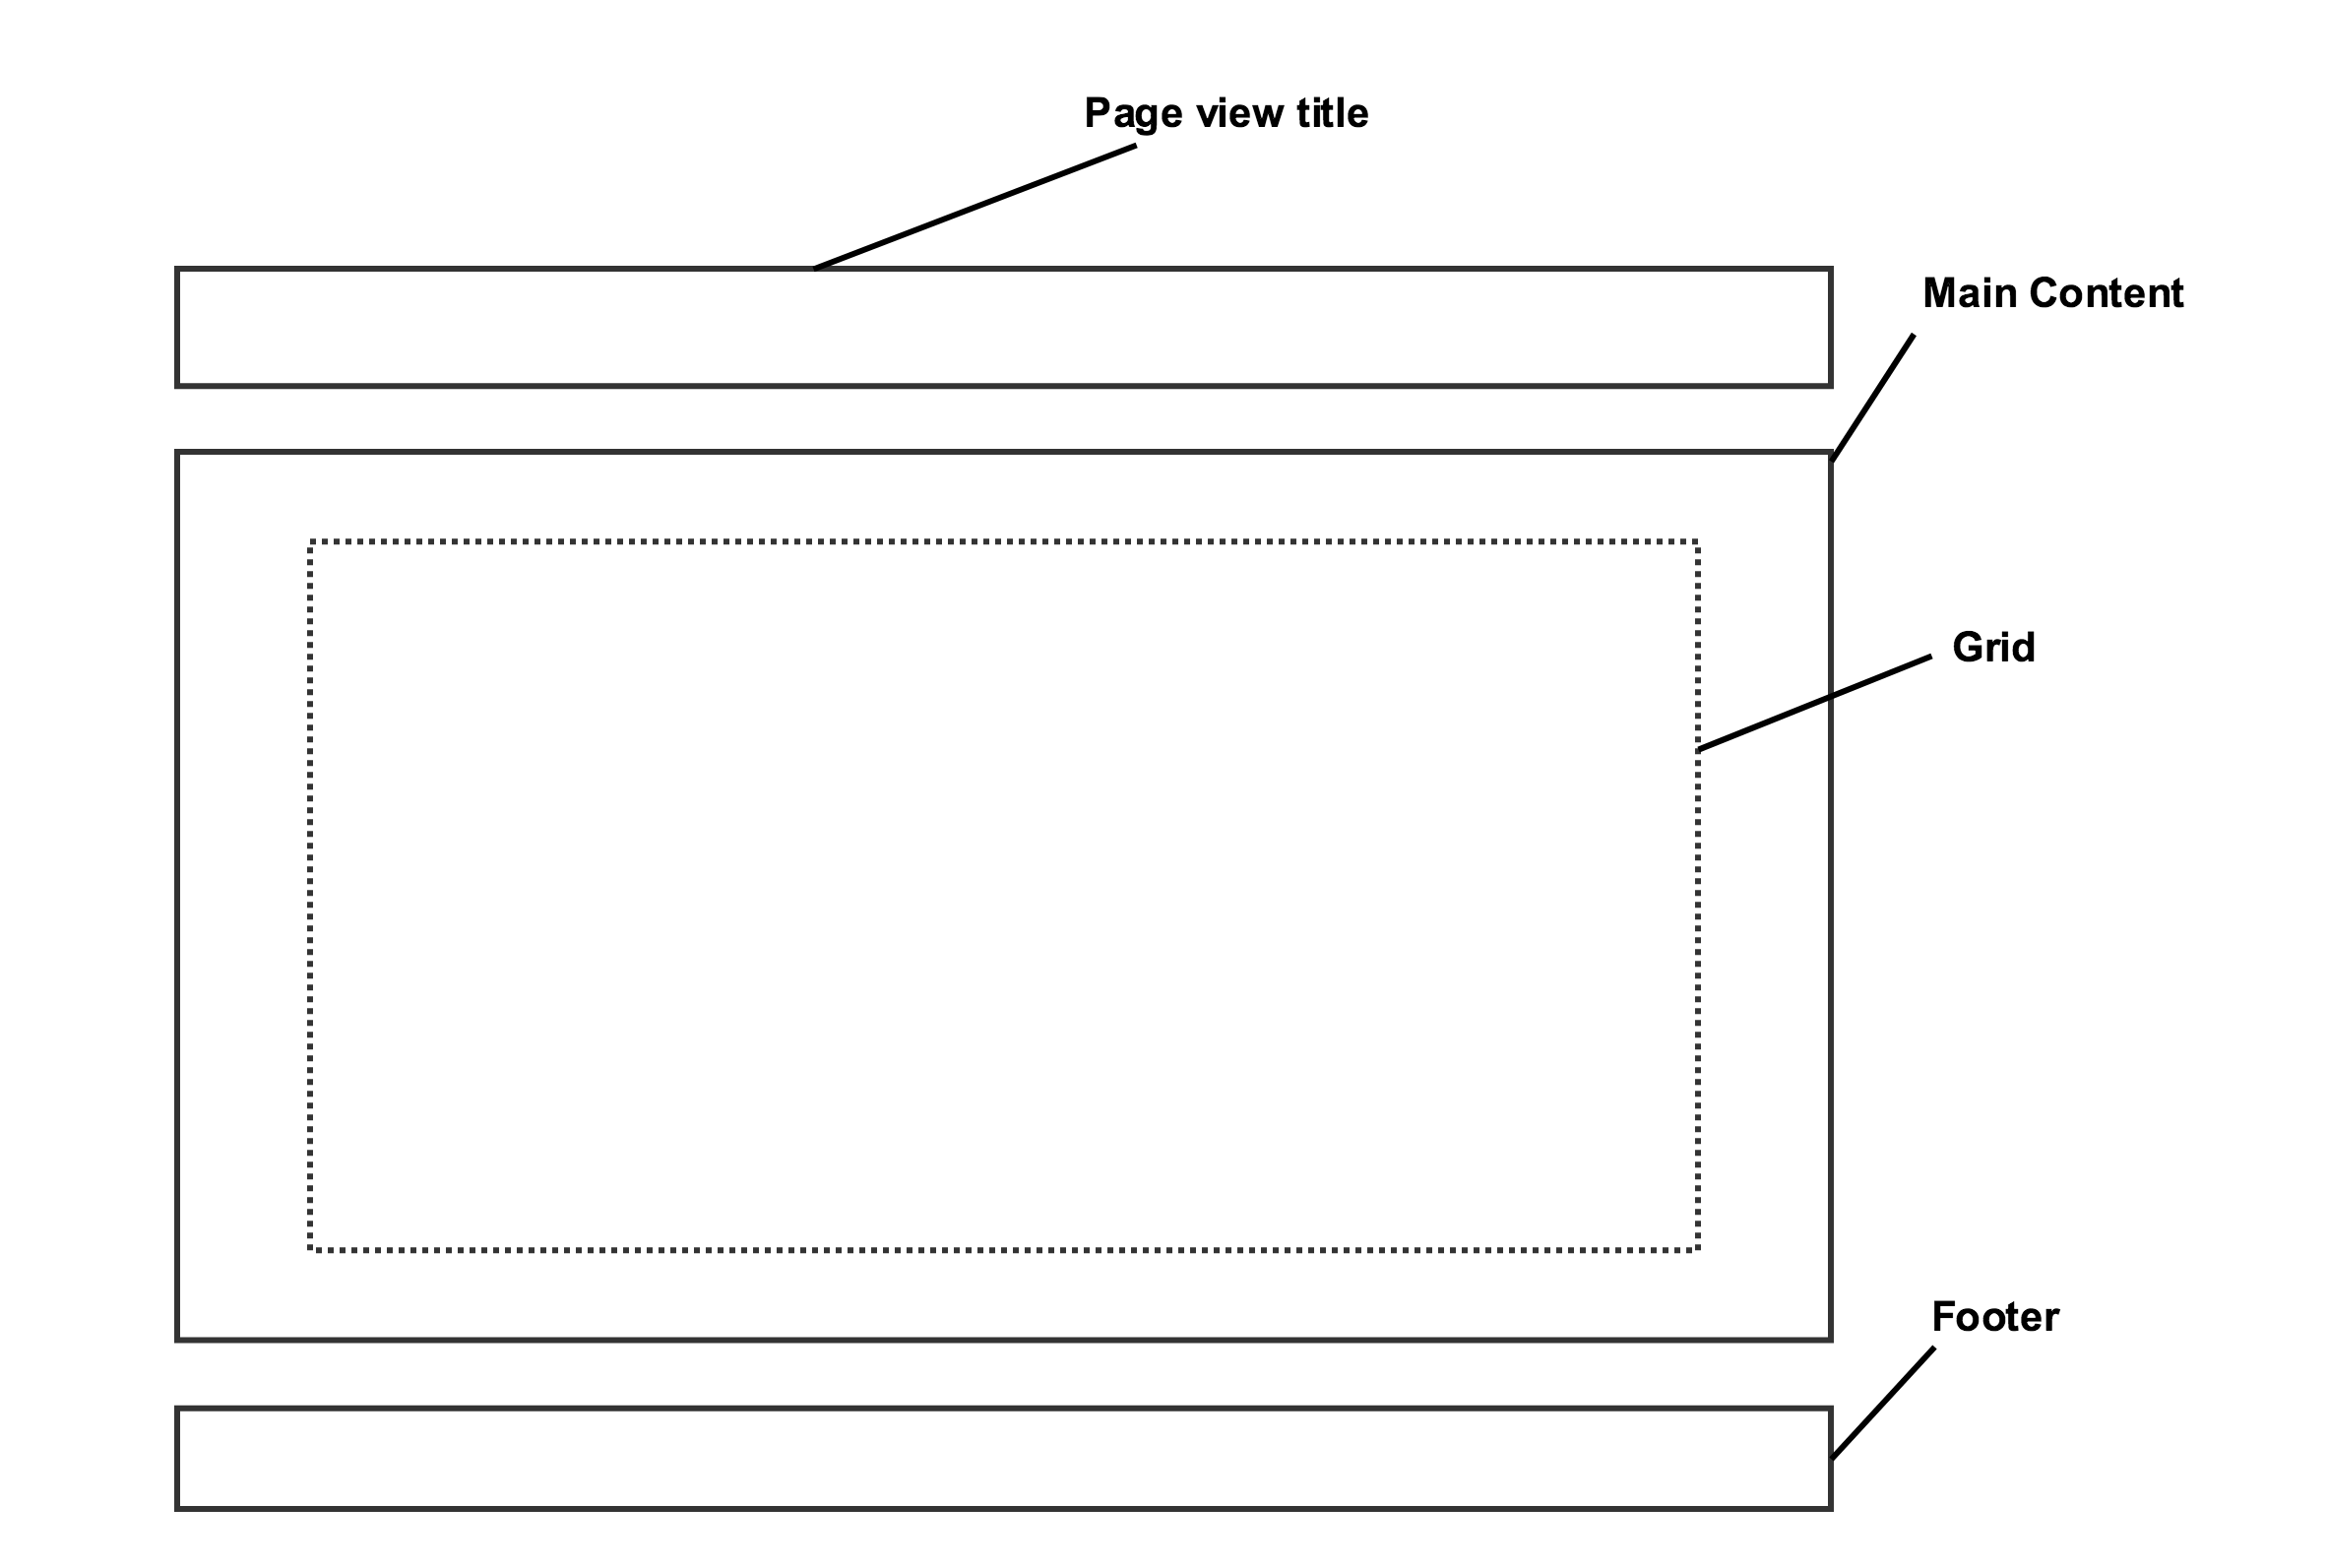
\includegraphics[width=\linewidth]{components/3/components/layout_basic.png}
  \caption{N2Sky Fundamental Layout}
  \label{fig:layout_basic}
\end{center}
\end{figure}

This layout applies styling like:
\begin{itemize}
\item Colors
\item Formatting
\item  Fonts
\item Positioning of elements and components
\end{itemize}



Fundamental Layout is a base layout which contains following elements:
\begin{itemize}
\item Page view title is a component with a caption and optionally an icon or push-to-action button
\item Main Content is a centered component, which represent the primary context. This component is always in focus by the user and can contain one or more grid components.
\item Grid in its basic layout represents the positioning of elements, which can be displayed inside it. In the basic layout, in grid components it is possible to add any elements. 
\item Footer is a component which goes across the whole application with a static data. Normally, it contains terms and conditions. 
\end{itemize}


\subsubsection{N2Sky Main Layout}\label{N2Sky Main Layout}

The N2Sky Main Layout, which is shown in ``Fig.~\ref{fig:layout_main}'',  is extending the N2Sky Fundamental Layout. Any changes in the basic layout will be automatically reflected in the main layout. Following components were added:

\begin{figure}[H]
\begin{center}
  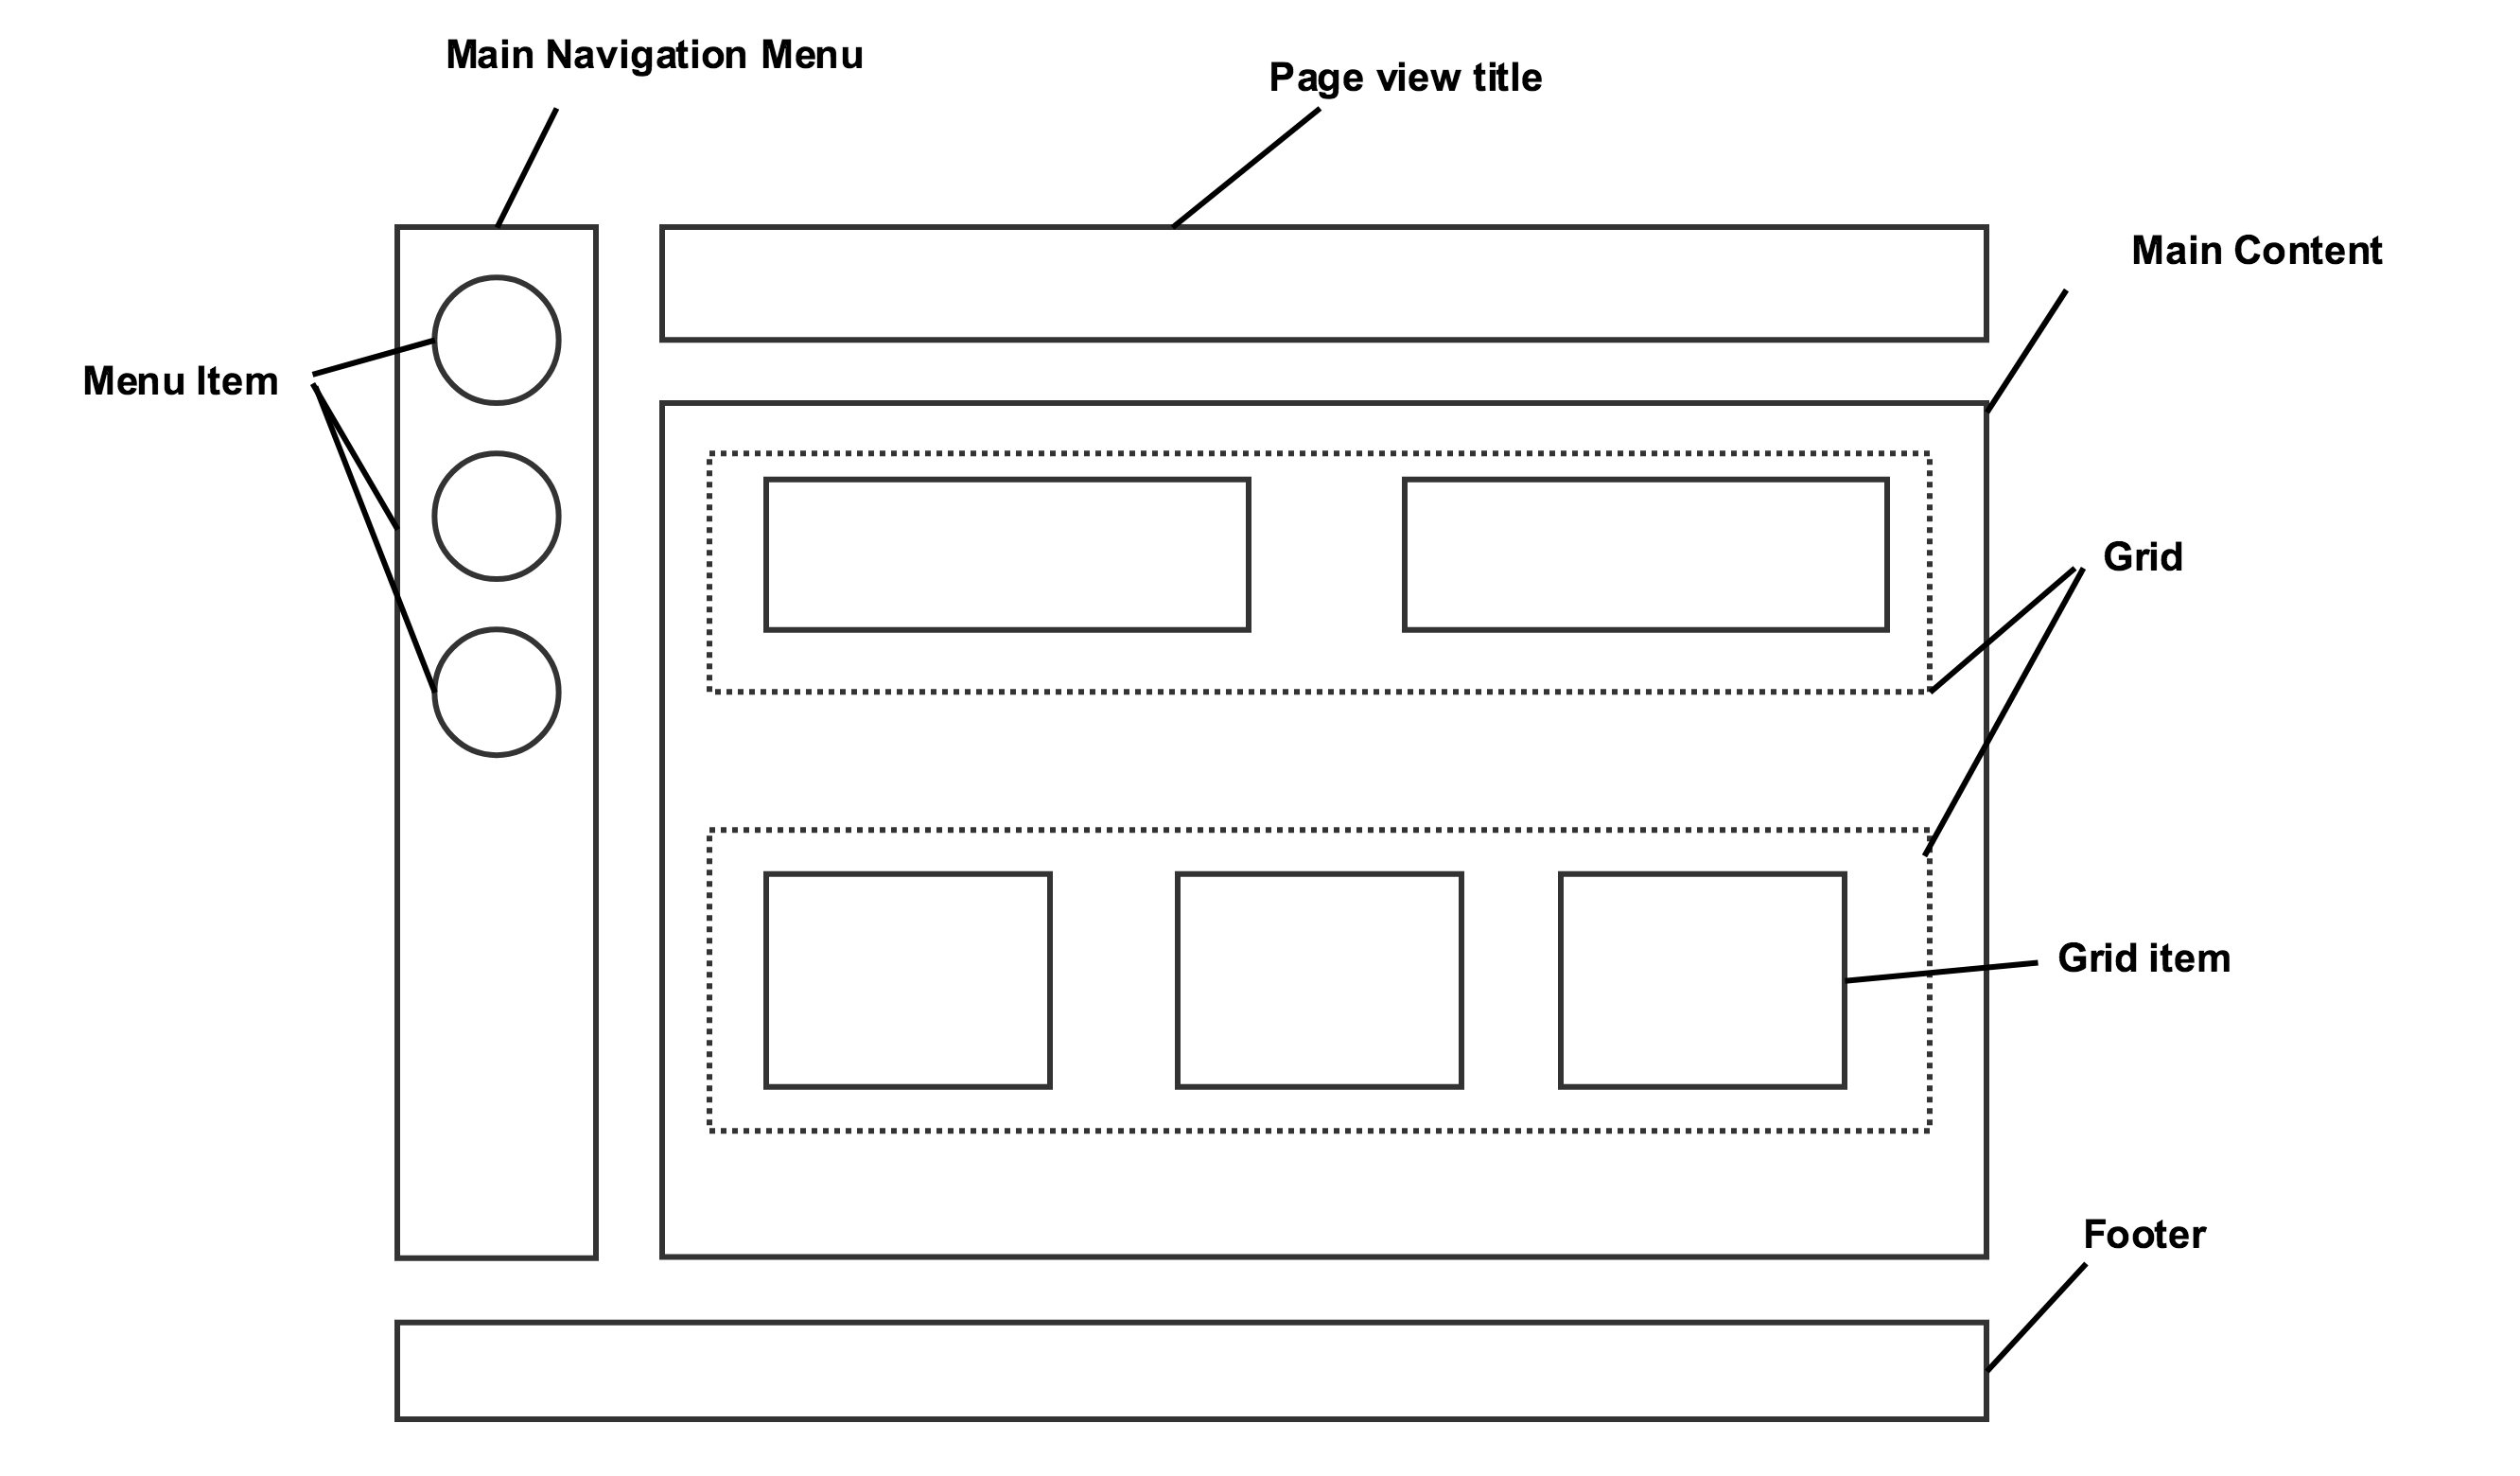
\includegraphics[width=\linewidth]{components/3/components/layout_main.png}
  \caption{N2Sky Main Layout}
  \label{fig:layout_main}
\end{center}
\end{figure}

\begin{itemize}
\item Main Navigation Menu, which is displayed as a vertical bar. This component has two states: on mouse over which it will be extended and menu items with caption text and icons will appear; on mouse away from the component only menu items icon will be displayed. 
\item Menu items are icons with caption components. Which items will be shown or hidden depends on the users permissions.
\item Grid items are blocking components, which can have multiple sizes but fixed within one grid. The context of grid items can be customized. 
\end{itemize}



\subsubsection{N2Sky Mobile Layout}\label{N2Sky Mobile Layout}

N2Sky supports mobile devices. For mobile devices, the mobile layout was developed as is shown in figure \ref{fig:layout_mobile}.

\begin{figure}[H]
\begin{center}
  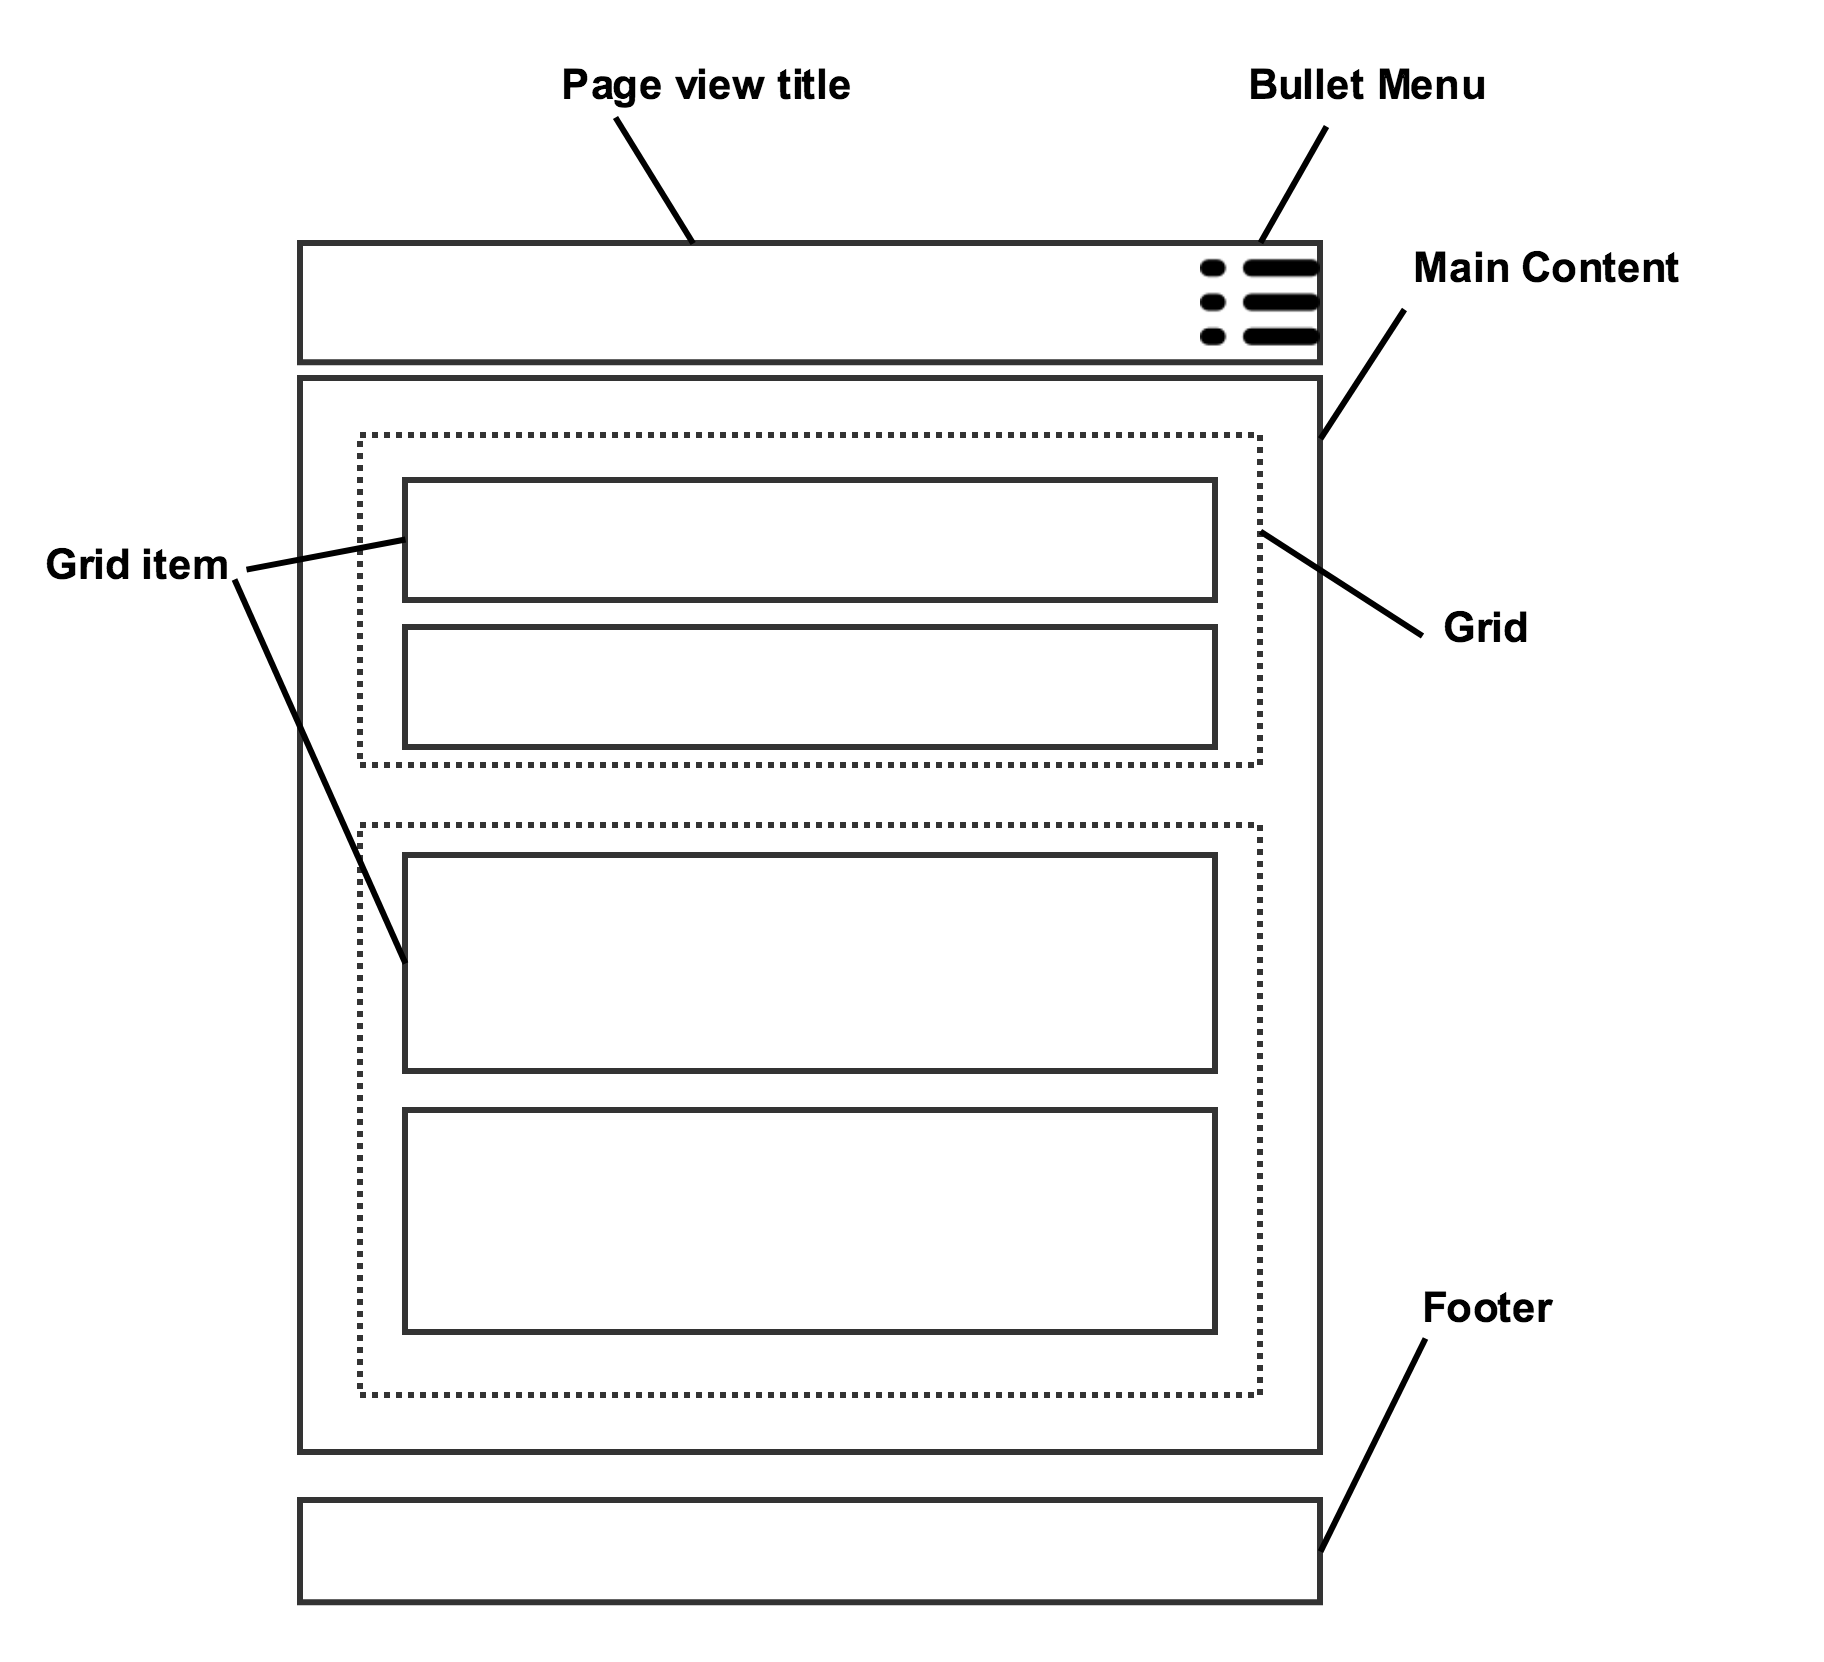
\includegraphics[width=\linewidth]{components/3/components/layout_mobile.png}
  \caption{N2Sky Mobile Layout}
  \label{fig:layout_mobile}
\end{center}
\end{figure}

The context of all components remains the same, but the positioning is changed. All grid items are vertically located and the width of grid items are the same as the device screen size. 

Additionally, next to the page view title component is the Bullet Menu located. The normal desktop view is hidden and instead the bullet menu will perform the same functionality. On click, the menu will appear as an overlay of the current view. 

\subsubsection{N2Sky Page Views}\label{N2Sky Page Views}

As it was mentioned in \autoref{Technology Stack} "Technology Stack", the N2Sky frontend application is developed on the ReactJS framework. An important part of the ReactJS framework is the React-Router, which contains all page views of the application and redirects it according to the URL path:

\begin{lstlisting}[caption=React Router]
<Provider store={store}>
	<Router history={browserHistory}>
		<Route path="/" component={Auth}/>
		<Route path="/signup" component={Reg}/>
		<Route component={AbstractDashboardLayout}>
			<Route path="/cloud" component={DashboardsOverview}/>
			<Route path="/user/profile" component={UserProfile}/>
			<Route path="/openstack" 
				component={OpenStackMainDashboard}/>
			<Route path="/openstack/project/:id"
				 component={OpenStackProjectDashboard}/>
			<Route path="/openstack/server/:projectid/:serverid" 
				component={ServerDetailsDashboard}/>
			<Route path="/openstack/vitrage/:templateId" 
				component={VitrageDetailsView}/>
			<Route path="/alert" component={AlertDashboard}/>
		</Route>
		<Route component={AbstractDashboardLayout}>
			<Route path="/n2sky" component={N2SkyDashboard}/>
			<Route path="/n2sky/available"
				 components={AvailableNetworksOverview}/>
			<Route path="/n2sky/models" 
				components={ModelsRepository}/>
			<Route path="/n2sky/paradigm/create/:projectid" 
				components={AddNNFromParadigm} readOnly={false}/>
			<Route path="/n2sky/paradigm/nn/:id" 
				components={AddNNFromParadigm} readOnly={true}/>
			<Route path="/n2sky/network/:id" 
				component={NetworkDetails}/>
			<Route path="/n2sky/network/:id/test/:model_id"
				 component={NetworkTestDetails}/>
			<Route path="/n2sky/project/:id"
				component={ProjectDashboard}/>
		</Route>
	</Router>
</Provider>
\end{lstlisting}

Every "Route" is a page view redirector and contains:
\begin{itemize}
\item Path, which is responsible for URL redirection.
\item Component, which is a page view itself
\item Other props, which are optional
\end{itemize}

As it was mentioned in \autoref{Modular frontend application design} "Modular frontend application design", N2Sky contains two modules: Administration module and main application module. Both of these modules are sharing the same main application layout and having following page views: 
\begin{itemize}
\item \textbf{Administration Module:}
\begin{description}
\item[Cloud Dashboard View, path: "/cloud".] It is the main dashboard of Administration module, which contains overview dashlets of every modules component.
\item[OpenStack Dashboard View, path: "/openstack".] This view contains all information about OpenStack and is the main control center of the OpenStack services.
\item[OpenStack Project, path: "/openstack/project/:id".] Route to the OpenStack project, which contains information about servers, flavours, images etc. of the particular project. In path "id" is the id of OpenStack project.
\item[Server Details View, path: "/openstack/server/:projectid/:serverid".] This view contains information about OpenStack instance. The URL path needs OpenStack project id and the id of the OpenStack instance. 
\item[Vitrage Details View, path: "/openstack/vitrage/:templateId".] Vitrage is a monitoring service of OpenStack and its instances. This view contains information about this service. The template id is required.
\item[Alert Management Dashboard View, path: "/alert".]  This view is a dashboard of the Alert Management System. This view contains information about alerting rules and alerting events.
\end{description}

\item \textbf{Main Application Module:}
\begin{description}
\item[Authentication View, path: "/".] First page in which the user sees when he is loading the application. Authentication View contains the login form.
\item[Registration View, path: "/signup".] Registration View contains the registration form.
 \item[N2Sky Dashboard, path: "/n2sky".] Main Application Module view is the N2Sky Dashboard. This view contains information about logged in user projects, neural networks and trained models.  
\item[Available Networks View, path: "/n2sky/available".] This view is the neural network repository of the N2Sky. It is possible to copy available neural networks to own projects.
\item[Models Repository View, path: "/n2sky/models".] The trained neural network are showed in this view. It is possible to copy published models to own projects.
\item[Neural Network Create View, path: "/n2sky/paradigm/create/:projectid".] This view represents the workflow of the creation of neural networks from existing paradigms. The newly created neural network will be saved in users project, hence this project id is required.  
\item[Neural Network Details View, path: "/n2sky/network/:id".] The details of the created neural network. It can be a logged in users neural network as well as the neural network of another user. User permissions show visibility levels. The networks id is required. 
\item[Neural Network Test View, path: "/n2sky/network/:id/test/:model\_id".] From this view, the user can evaluate neural networks with his own input parameters. Neural network id and trained model id are required. 
\item[Project Dashboard View, path: "/n2sky/project/:id".] This view shows the neural networks and models, which were created in a particular project. The project id is required.
\end{description}


\end{itemize}






\subsubsection{N2Sky Dashboards}\label{N2Sky Dashboards}

The purpose of the dashboard is to embed business intelligent (BI) objects into a single page in order to make an overview of highlighted titles of BI objects \cite{dashboards_book}.

A dashboard has a structure layer upon its dashlets. It allows the user to manage layout and properties of dashlets. A dashboard is composed of dashlets. Every dashlet contains specific context and data. A dashboard defines: 
\begin{itemize}
\item Dashlets to be displayed
\item The layout of dashboard and positioning of its dashlets
\item The common context of particular dashlets
\end{itemize}


\begin{figure}[H]
\begin{center}
  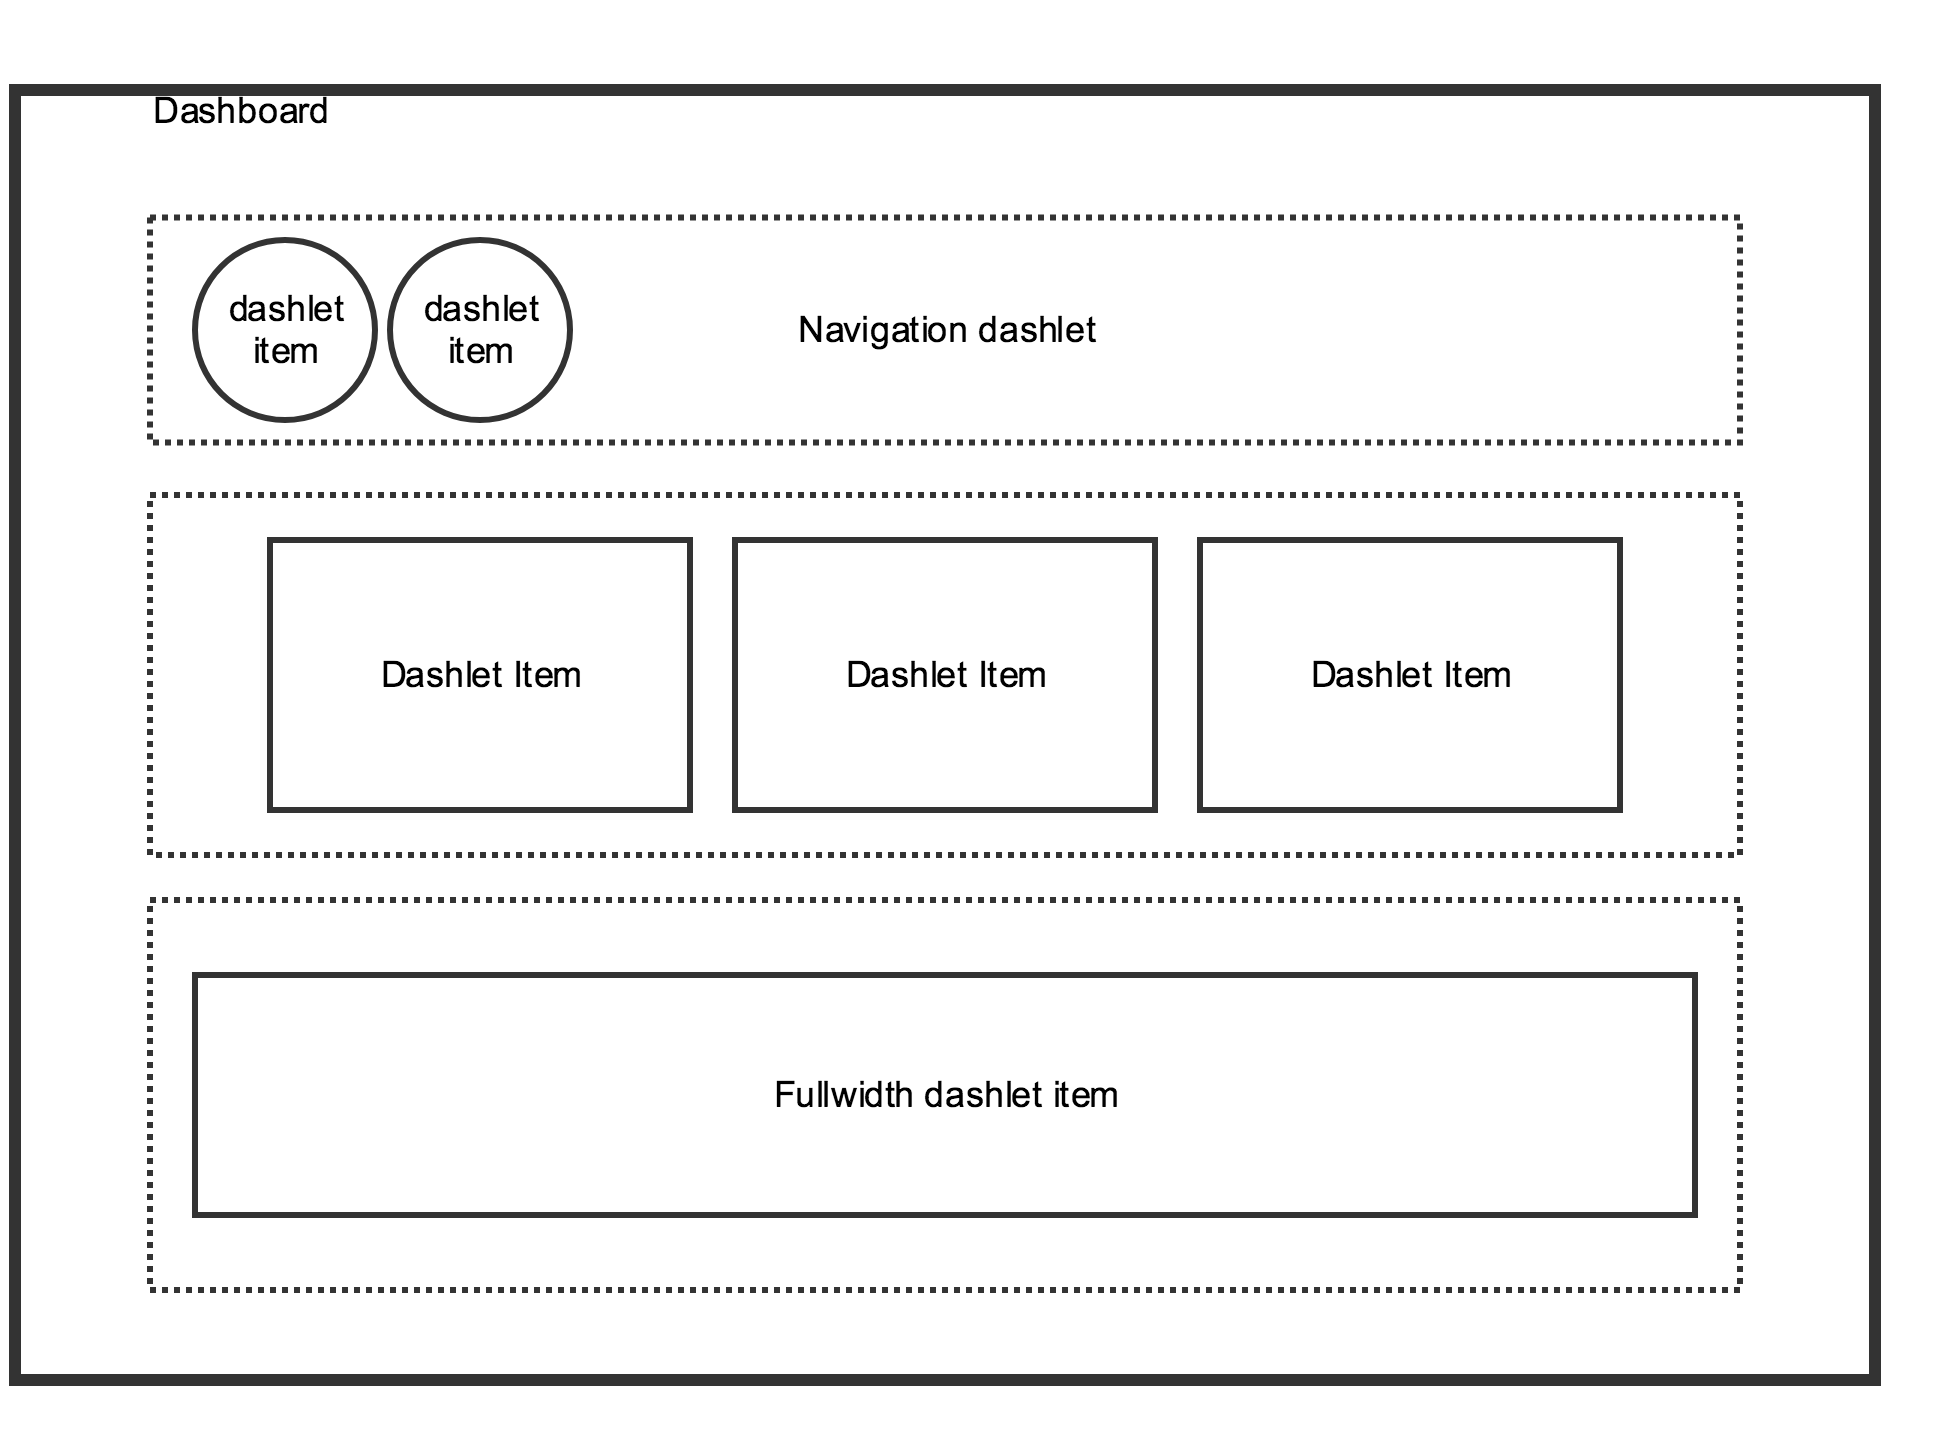
\includegraphics[width=\linewidth]{components/3/components/dashboard_template.png}
  \caption{N2Sky Dashboard template}
  \label{fig:dashboard_template}
\end{center}
\end{figure}

In the figure \ref{fig:dashboard_template} is shown the typical N2Sky dashboard template. A dashboard in N2Sky has a grid structure. Every dashlet has one or more items. Each item can contain any UI component, but it has to be fit into assigned dashlet without overlays. 



\subsubsection{Responsive Design}\label{Responsive design}

Since N2Sky is cross-platform application, it has to support multiple screen resolutions as well as readability and usability. 

Considering readability, first of all the typography has to be mentioned. During the development of N2Sky, a confronted challenge was when choosing from different usable fonts, which would be displayed all the same and be readable across multiple devices. The typeface \cite{wiki:typeface} properties like latter spacing, width, weight etc were adjusted multiple times. The common problem was to audit how typeface represents on mobile devices and desktop computers \cite{responsive_book}. Even such standard fonts like "Arial" and "Times New Roman" appeared unreadable on mobile devices as shown in figure \ref{fig:typo}.

\begin{figure}[H]
\begin{center}
  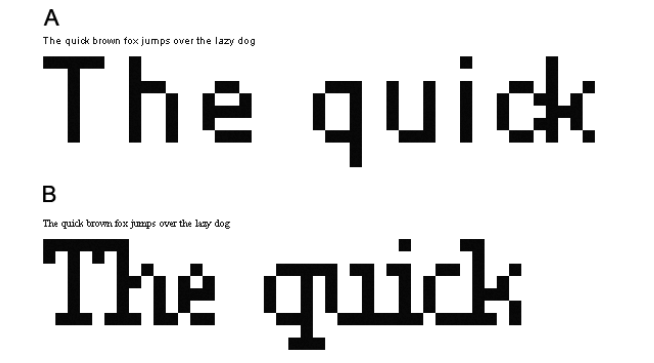
\includegraphics[scale=0.5]{components/3/components/typo.png}
  \caption{Difference between sans-serif font Arial (A) and the browser serif font Times New Roman (B) }
  \label{fig:typo}
\end{center}
\end{figure}

The expansion of cross-platform applications brought freedom to developers and designers. Today is possible to develop an application simultaneously for mobile devices, desktop computers, and web browsers. Problems were though faced when the mobile and tablet devices manufacturers started to produce devices with different resolutions. Today, the versioning of mobile screen resolution came to over 1000 devices, but N2Sky was concentrating only on major market players as shown in figure \ref{fig:screen} \cite{mobile_resolution}.

\begin{figure}[H]
\begin{center}
  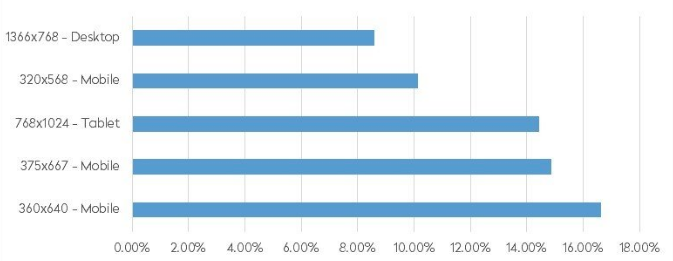
\includegraphics[scale=0.65]{components/3/components/screen.png}
  \caption{Average screen resolution of mobile, tablet and desktop devices on 2017}
  \label{fig:screen}
\end{center}
\end{figure}

N2Sky is focused on mobile and tablet devices because of the extensive trend nowadays. 

\subsubsection{User Interface Elements}\label{User Interface Elements}

It is possible to divide all UI elements into groups \cite{intelligent_support}:

\begin{description}
\item[Input Controls.] Input controls determine user input action. Input actions are keyboard typing or mouse clicking. Following UI elements are the part of input controls: 
\begin{itemize}
\item Checkboxes
\item Radio buttons 
\item Dropdown Lists
\item List boxes
\item Buttons
\item Toggles
\item Text fields
\item Date field
\end{itemize}
\item[Navigational Components.] Navigation between page views. Navigational components include also some particular request from and to users. Following UI elements are the parts of navigational components:
\begin{itemize}
\item Breadcrumb 
\item Slider
\item Search field
\item Pagination
\item Slider
\item Tags
\item Icons
\end{itemize}
\item[Informational Components.] These components are the addition to workflows. It can help the user to perform actions or inform him that the action will occur or has already occurred. Informational Components contain following UI elements:
\begin{itemize}
\item Tooltips
\item Icons
\item Progress bar
\item Notifications
\item Message boxes
\item Modal windows
\end{itemize}
\item[Containers.] Containers are components, which are hiding additional information or not focused information, where the user needs to perform the action in order to see it.   
\begin{itemize}
\item Accordion
\item Semi-hidden elements
\end{itemize}
\end{description}

\subsubsection{UI Elements in N2Sky}\label{UI Elements in N2Sky}

N2Sky supports almost all common web user interface elements. Every element was developed in order to be reusable. Since N2Sky supports responsive design, the UI elements should also be responsive. Each of the UI elements is absolutely customised. Following UI elements were created:

\begin{description}
\item[Accordion]  Accordion is a list of items, which is accessible on mouse click. The N2Sky accordion works more or less like a modal window. With this kind of functionality, other data, which surround the accordion will not be stretched or squeezed but appear on top of elements as shown in figure \ref{fig:accordion}: 

\begin{figure}[htbp]
\begin{center}
  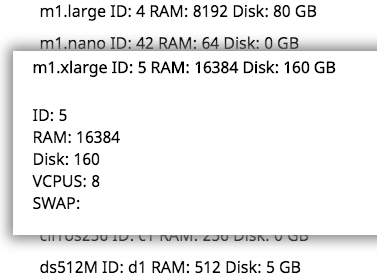
\includegraphics[scale=0.75]{components/3/components/accordion.png}
  \caption{Customised N2Sky accordion UI element}
  \label{fig:accordion}
\end{center}
\end{figure}

\item[Buttons.] The idea behind it was to make buttons more interactive and understandable to use as displayed in \ref{fig:button_inactive}. Buttons contain a caption and icon in SVG format in order to support high quality image in all devices.

Buttons are using on hover animation. When the mouse moves over a button, then the icon slides in the middle to show that the action can be performed as shown in figure \ref{fig:button_active}. 

\begin{figure}[htbp]
\begin{center}
  
\includegraphics[scale=0.55]{components/3/components/button_inactive.png}
  \caption{Customised N2Sky button UI element}
  \label{fig:button_inactive}
\end{center}
\end{figure}


\begin{figure}[htbp]
\begin{center}
  
\includegraphics[scale=0.55]{components/3/components/button_active.png}
  \caption{Customised N2Sky button UI element animation}
  \label{fig:button_active}
\end{center}
\end{figure}

\item[Icons.] In N2Sky, all icons are in Scalable Vector Graphics (SVG) format. With SVG the icons do not loose their quality in any device \cite{Cagle2005}. Since it is a vector graphic, it is easy to edit an icon with programming language code. The N2Sky Logo, which is represented in figure \ref{fig:logo}, also uses the SVG format. 

\begin{figure}[htbp]
\begin{center}
  
\includegraphics[scale=0.55]{components/3/components/logo.png}
  \caption{Customised N2Sky logo in SVG format}
  \label{fig:logo}
\end{center}
\end{figure}

Importing code in some graphical vector editor in order change color, path (vector graphic itself), metadata etc is also possible. The following code demonstrates the N2Sky Logo in SVG format. The whole vector path was shortened.

\begin{lstlisting}[language=XML, caption=SVG example]
<?xml version="1.0" standalone="no"?>
<!DOCTYPE svg PUBLIC "-//W3C//DTD SVG 20010904//EN"
        "http://www.w3.org/TR/2001/REC-SVG-20010904/DTD/svg10.dtd">
<svg version="1.0" xmlns="http://www.w3.org/2000/svg"
     width="266.000000pt" height="267pt" viewBox="0 0 266 267"
     preserveAspectRatio="xMidYMid meet">
    <metadata>
        N2Sky Logo. 2018
    </metadata>
    <g transform="translate(0.000000,267.000000) scale(0.100000,-0.100000)"
       fill="#6b6b6b" stroke="none">
        <path d="M1302 2638 c-9 -9 -12 -83 -12 -270 0 -245 -1 -259
-37 -26 -170 21 -63 23 -132 46 -152 52 -23 7 -38 17 -38 27 1
80 222 90 255 87 284 -2 23 -9 32 -25 34 -27 4 -46 -23 -72 -106 
-77 -34 -95 -8 -18 -22 -51 -32 -74 -10 -24 -21 -43 -25 -43 -5 0 -30 
76 -76 118 -100 136 -128 92 -12 -20 -10 -26 101 -219 35 -60 109 

...

-18 74 -40 36 -22 67 -40 70 -40 11 0 253 -152 269 -169 11 -12 15 -27 12 
-36 26 -103 -14 -32 -19 -60 -35 -62 -35 -3 0 -34 -18 -70 -40 -36 -22 -68
-40 -70 -40 -3 0 -22 -11 -43 -23 -142 -90 -172 -96 -201 -39 -20 40 -47 168
-55 268 l-5 61 122 22 c67 13 156 30 197 38 85 16 106 30 95 63 -7 21 -11 22
-69 16 -33 -4 -88 -10 -121 -15 -178 -26 -178 -26 -170 -1 4 13 21 46 37 74
57 100 63 116 52 134 -6 9 -22 17 -34 17 -24 0 -47 -33 -130 -180 -75 -132
-74 -130 -61 -206 6 -38 16 -102 21 -141 6 -40 15 -98 20 -129 6 -30 10 -72
10 -93 l0 -38 -162 4 c-151 3 -167 5 -212 28 -82 43 -86 57 -86 320 l0 226 38
34 c21 19 53 47 72 61 19 14 49 39 67 55 17 16 54 47 82 69 60 49 79 79 65
103 -18 28 -47 25 -84 -10 -20 -18 -52 -45 -72 -60 -20 -15 -42 -34 -50 -41
-23 -23 -92 -67 -105 -67 -10 0 -13 27 -13 104 0 57 -3 111 -6 120 -7 19 -45
21 -62 4z"/>
    </g>
</svg>
\end{lstlisting}

\item[Notification messages.] Notification messages are part of the information component. In N2Sky, there are used two types of notification messages: 
\begin{itemize}
\item Warning messages, which announce that something goes wrong as shown in ``Fig.~\ref{fig:notif_warning}''. It can be an error in the application or an user workflow error. 
\item Informational messages give information about the event which will occur or already occurred as shown in ``Fig.~\ref{fig:notif_info}''.
\end{itemize}


\begin{figure}[htbp]
\begin{center}
  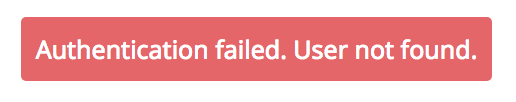
\includegraphics[scale=0.65]{components/3/components/notif_warning.png}
  \caption{Customised N2Sky warning message UI element}
  \label{fig:notif_warning}
\end{center}
\end{figure}

\begin{figure}[htbp]
\begin{center}
  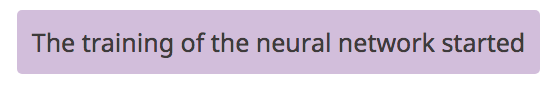
\includegraphics[scale=0.65]{components/3/components/notif_info.png}
  \caption{Customised N2Sky informational message UI element}
  \label{fig:notif_info}
\end{center}
\end{figure}

\item[Navigation.] In N2Sky, a user can navigate to another page or change part of the page view via tabs, navigation buttons, and menus. 
Navigation elements are bind to the group of element or UI components. The following navigation component which is shown in ``Fig.~\ref{fig:nav}'', contains navigation elements as well functional icons. 
\end{description}

\begin{figure}[htbp]
\begin{center}
  
\includegraphics[scale=0.65]{components/3/components/nav.png}
  \caption{Customised N2Sky navigation UI element}
  \label{fig:nav}
\end{center}
\end{figure}

Navigation bars can contain tabs, buttons, icons and non-functional text. ``Fig.~\ref{fig:nav_bar}'' shows the navigation bar of a custom table. 

\begin{figure}[htbp]
\begin{center}
  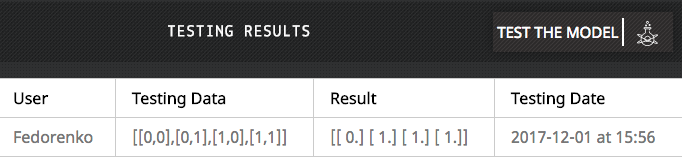
\includegraphics[scale=0.65]{components/3/components/nav_bar.png}
  \caption{Customised N2Sky navigation bar with a table}
  \label{fig:nav_bar}
\end{center}
\end{figure}

\subsubsection{UI Components in N2Sky}\label{UI Components in N2Sky}

Groups of UI elements form UI components. Components, like elements, are also fully reusable, the only context of components is changing. Following custom UI components were developed in N2Sky: 

\begin{description}
\item[Grid Item Component.] Grid in N2Sky is responsive. It can change positions and size of grid items like shown in ``Fig.~\ref{fig:grid_item}''. 

\begin{figure}[htbp]
\begin{center}
  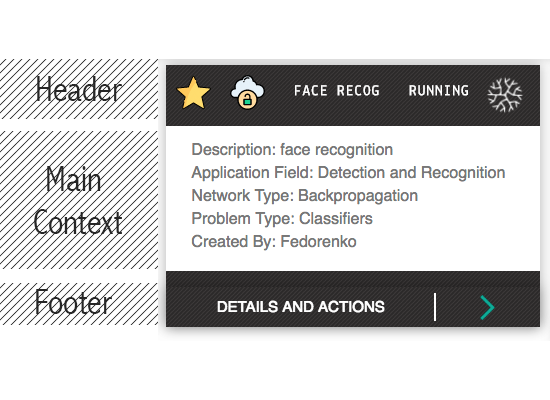
\includegraphics[scale=0.65]{components/3/components/grid_item.png}
  \caption{Responsive N2Sky Grid Item UI comonent}
  \label{fig:grid_item}
\end{center}
\end{figure}


Grid item contains following UI elements: 
\begin{description}
\item[Header. ] The first component on which the user focuses, that is why it should be short but highlighted. Following UI elements are included: 
\begin{itemize}
\item Functional icons-buttons on the left side (optional)
\item Title of grid item (mandatory)
\item  Non-functional icons (optional)
\end{itemize}
\item[Main context. ] Component, which contains context information. This component can be fully customized. It is possible to put list of items, plain text or even image.
 \item[Footer. ] Optional element and contains only the button UI element. 
\end{description}

\item[Main navigation menu.] Every N2Sky view uses a main navigation menu. The menu is injected in an abstract view, which is extended by all other view components. The menu has menu items, which contain a caption and an icon. As it was mentioned before, N2Sky has two modules: administration module and main application module. Both modules are represented in the menu and the menu items visibility depends on the logged-in users permission. 
The menu for arbitrary user is shown in figure \ref{fig:menu_user}  and has following menu items:

\begin{itemize}
\item Profile 
\item N2Sky Dashboard
\item Available neural networks
\item Models repository
\end{itemize}

 
 \begin{figure}[H]
\begin{center}
  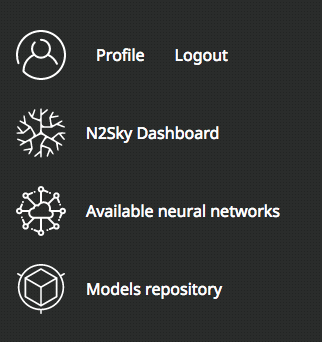
\includegraphics[scale=0.5]{components/3/components/menu_user.png}
  \caption{N2Sky Main Navigation Menu for arbitrary user}
  \label{fig:menu_user}
\end{center}
\end{figure}

If the end-user is a system administrator, an additional menu form administration module will appear as demonstrated in figure \ref{fig:menu_admin}. This menu contains dropdown submenus: 

\begin{itemize}
\item OpenStack Dashboard
\item Cloudify Dashboard
\item Alert System
\item Dashboards Settings
\end{itemize}


 \begin{figure}[H]
\begin{center}
  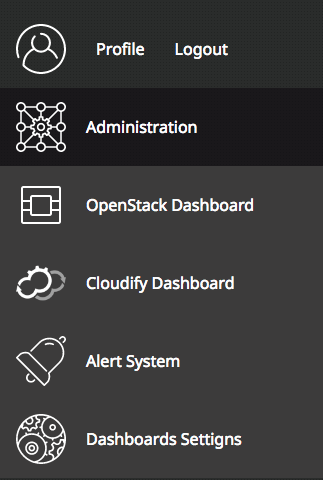
\includegraphics[scale=0.5]{components/3/components/menu_admin.png}
  \caption{N2Sky Main Navigation Menu for system administrator}
  \label{fig:menu_admin}
\end{center}
\end{figure}

\item[Modal windows.] N2Sky uses modal windows almost in every view as shown in figure \ref{fig:modal}. Modals are responsive and touch screen friendly. It has 3 elements:
\begin{itemize}
\item Title (mandatory)
\item Context (mandatory)
\item Submit button (optional)
\end{itemize}

 \begin{figure}[H]
\begin{center}
  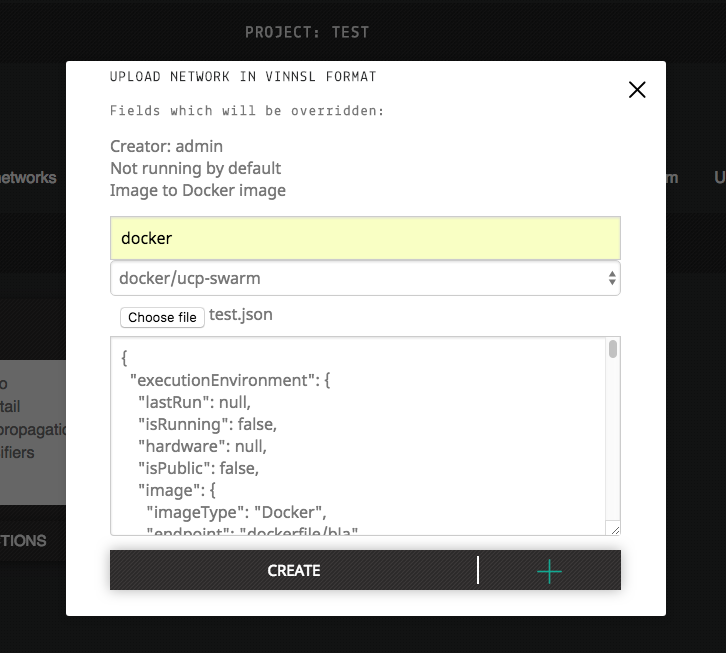
\includegraphics[scale=0.5]{components/3/components/modal.png}
  \caption{N2Sky Modal Window UI component}
  \label{fig:modal}
\end{center}
\end{figure}

Modals can be used to represent forms as well as for informational purposes. When a modal is open, the background is dunned in order to focus the user on its context. The modal context itself can be fully custom. It is possible to put any UI element in context.



\end{description}



\subsection{N2Sky Services}\label{N2Sky Services}

 N2Sky implements the microservices architecture. It has three main web services as shown in figure \ref{fig:newarch}:
 
\begin{itemize}
\item User Management Web Service
\item Model Repository Web Service
\item Cloud management Web Service
\end{itemize}

Every web service uses other services which are not exposed to the public. It was organised this way in order to support application encapsulation. Encapsulation of web applications helps to prevent security issues. One of the crucial processes in N2Sky is the neural network training. This process takes almost all resources of the environment, that is why it is unexposed. Such a process can be triggered only by a web service, which can be blocked if the environment is overloaded.

The above mentioned web services and also the processes and services that they encapsulate are in detail described:  


\subsubsection{User Management Web Service.}\label{User Management Web Service}   This web service is responsible for permissions and user management. It has its own database. The user can authorize the system and get a session token. Every token is a unique collection of numbers and Latin letters. The token is assigned to the authorized user and will be saved until the user is active. If the user is not active in the next 3 hours, the session token will disappear. If the user still has an active browser session, the authorization token will be revalidated. If the user is trying to make an illegal request or appears to have an overly active behaviour, the authorization token will be revoked and the system administrator will be notified of this incident. 

Every user encapsulates permission levels. There two different types of permissions:
\begin{itemize}
\item Administrator permission. The user has fully granted permission through the entire application.
\item Regular permission. The user has access only for his own as well as publicly available resources.  
\end{itemize}

 \begin{figure}[H]
\begin{center}
  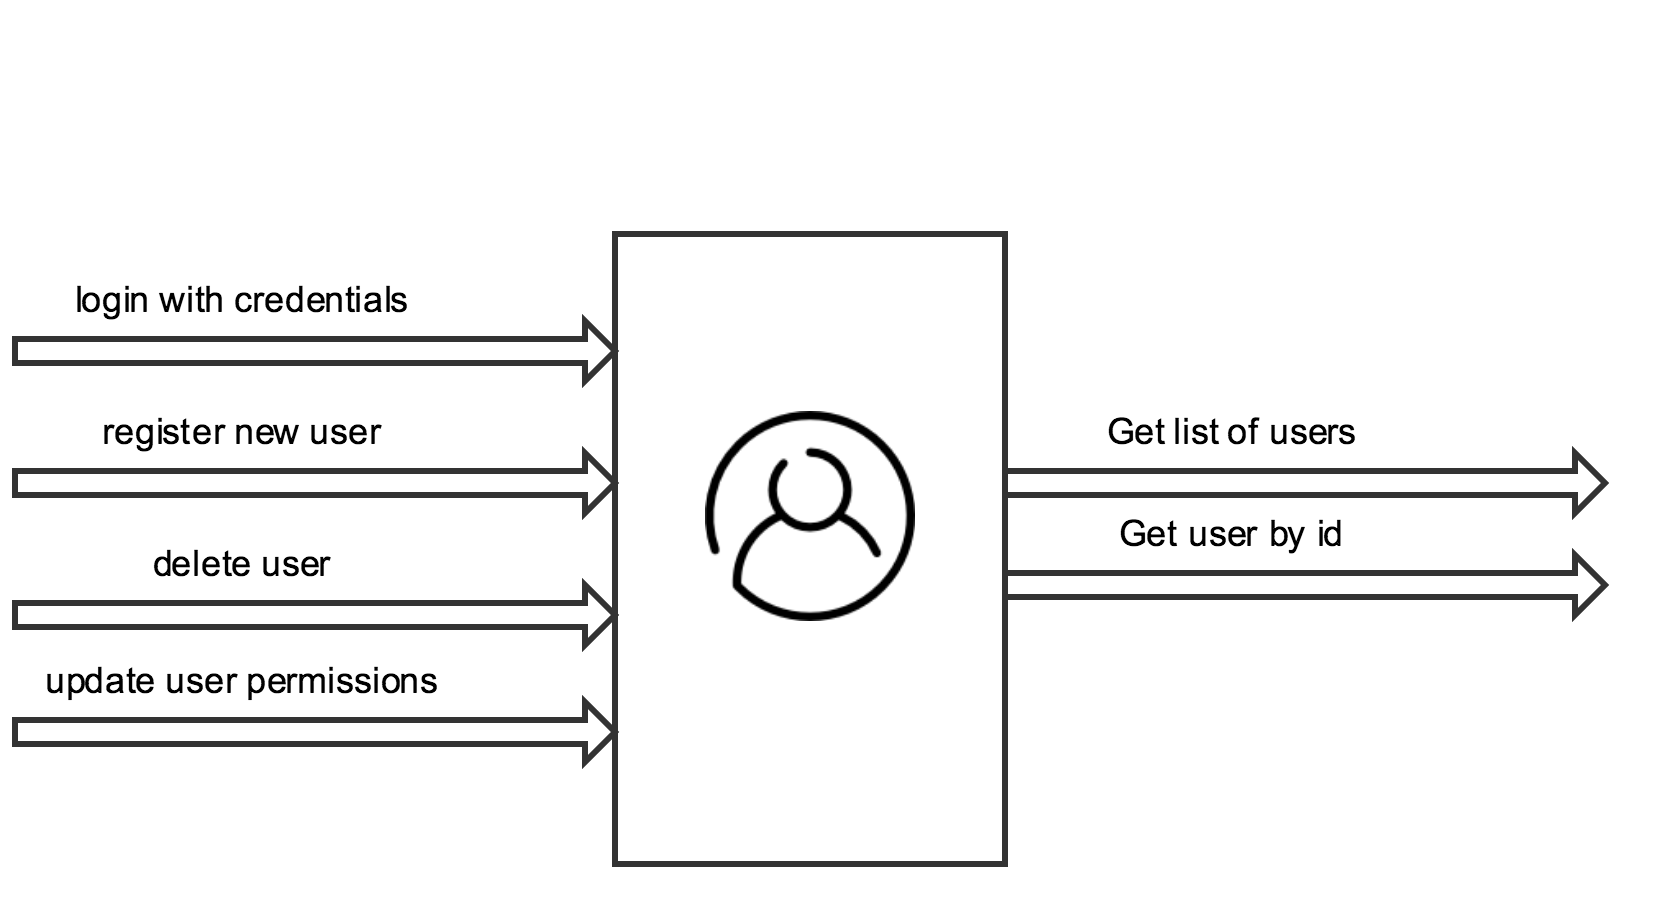
\includegraphics[width=\linewidth]{components/3/components/user_serivice.png}
  \caption{N2Sky User Management Web Service}
  \label{fig:user_serivice}
\end{center}
\end{figure}

As shown in ``Fig.~\ref{fig:user_serivice}'' User Management Web Service has following accessible services:

\begin{itemize}
\item Login with credentials
\item Register a new user 
\item Delete user
\item Update user permissions
\item Get list of users
\item Get user by user ID
\end{itemize}
 
Detailed information about web service API and API documentation can be found in \autoref{API Documentation}

\subsubsection{Model Repository Web Service.}\label{Model Repository Web Service}  Model Repository Web Service is the core service of N2Sky. The authorized user can create a new project, add their neural network from a chosen paradigm or deploy his own one. Every newly created project is assigned to one user and can not be shared. Only the system administrator can look up into other users projects. This functionality is also limited by User Management Web Service. 

Using this service, the user can create a neural network from proposed paradigms as well as upload his own neural network in the ViNNSL format \cite{Beran2008}. This functionality is exposed via the service so that each user can use it either from N2Sky web portal or via HTTP request directly on web service.

\begin{figure}[H]
\begin{center}
  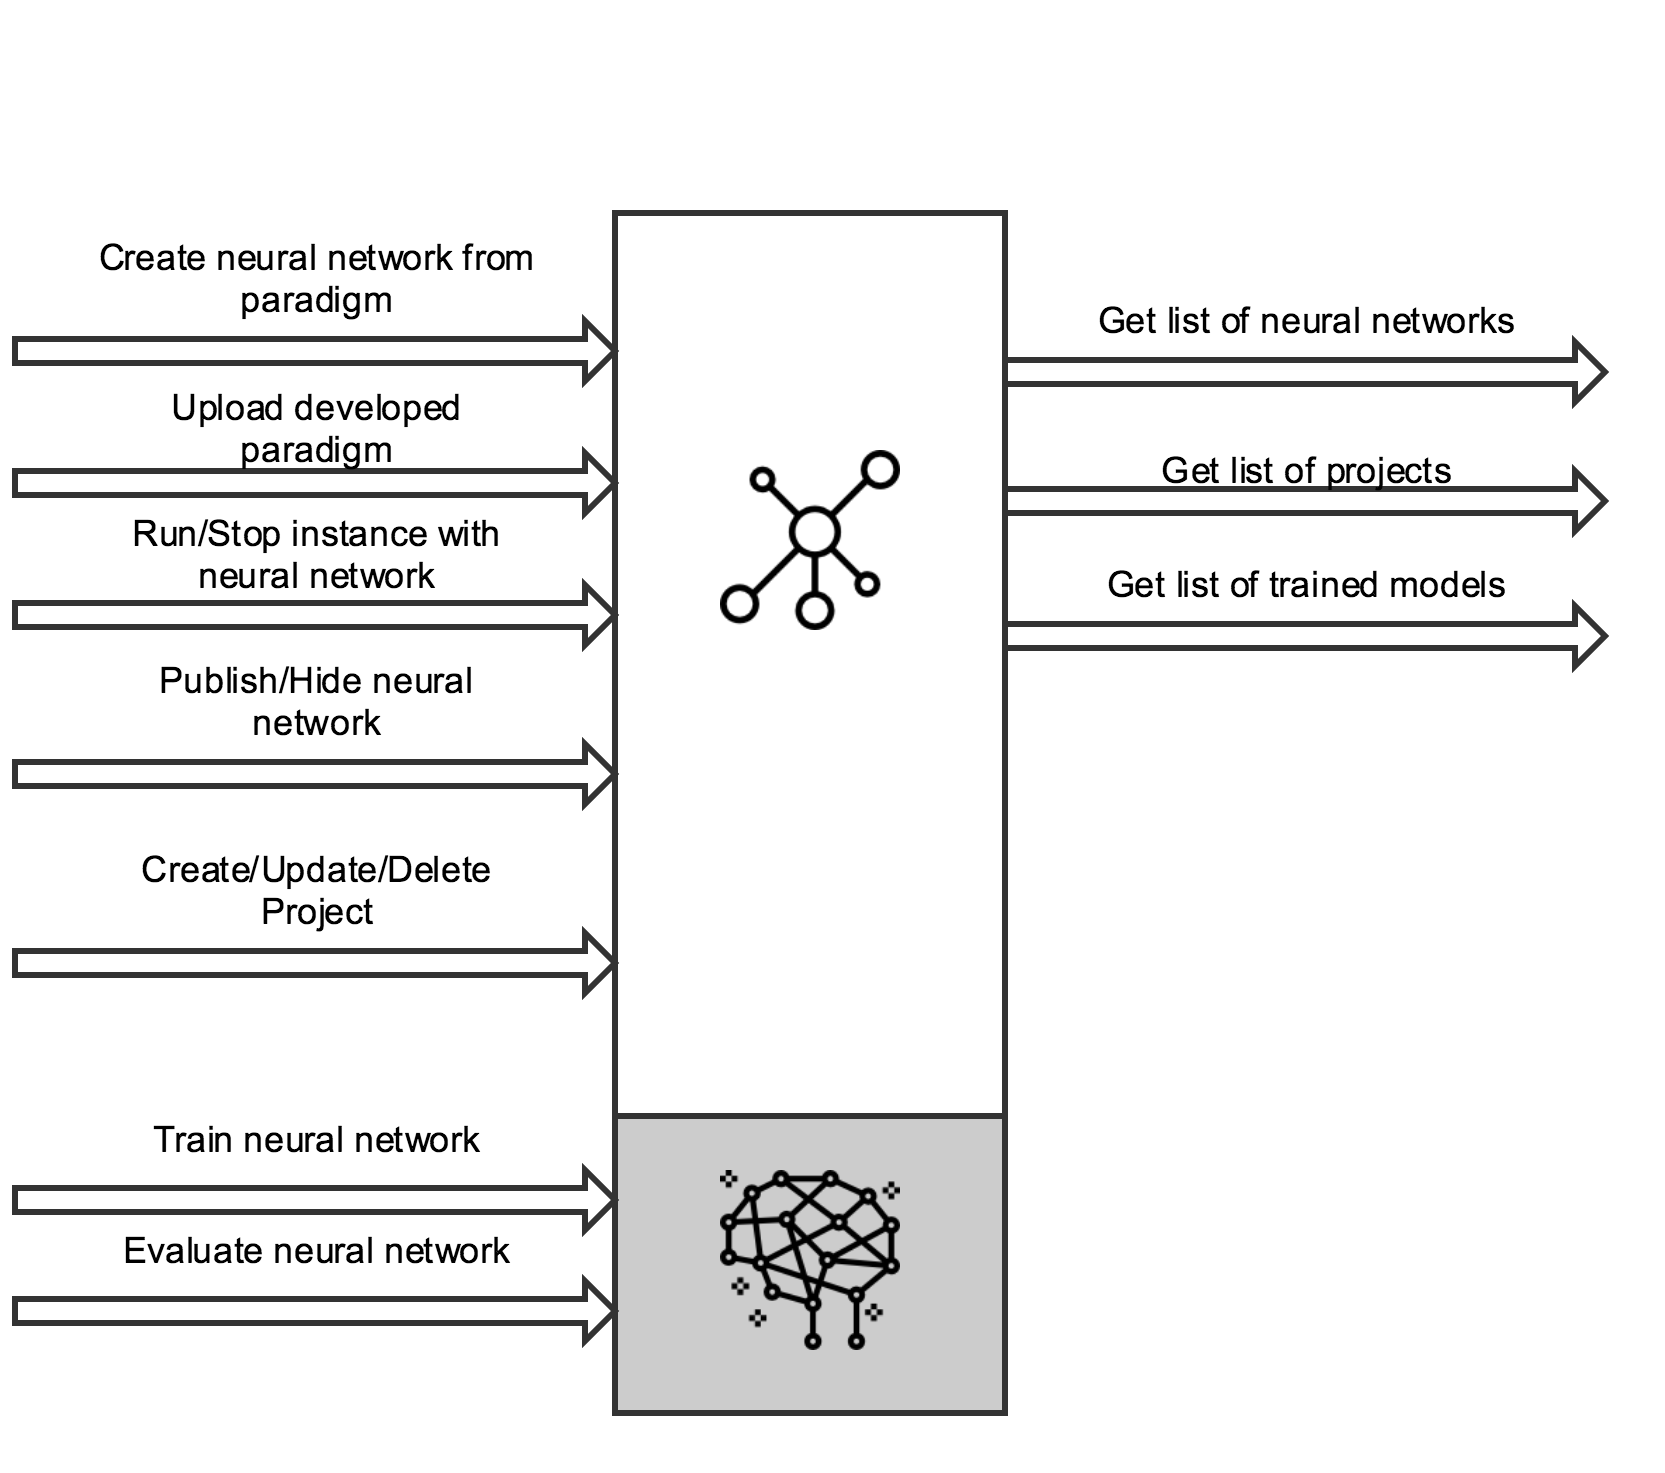
\includegraphics[width=\linewidth]{components/3/components/model_serivce.png}
  \caption{N2Sky Model Repository Web Service}
  \label{fig:model_serivce}
\end{center}
\end{figure}

As shown in figure \ref{fig:model_serivce} Model Repository Web Service has following accessible services:

\begin{itemize}
\item Create neural network from paradigms
\item Upload developed neural network paradigms
\item Run/Stop instances of neural networks
\item Publish/Hide neural networks 
\item Create/Update/Delete Project with neural networks
\item Get list of neural networks
\item Get list of projects
\item Get list of trained models 
\item Train neural networks (accessible only for the model management service itself)
\item Evaluate neural networks (accessible only for the model management service itself)
\end{itemize}

Detailed information about web service API and API documentation can be found in \autoref{API Documentation}


There are two services embedded in the Model Repository web service and not exposed:

\begin{description}
\item[Training service.]  This service provides the neural network training functionality. It is not possible to perform training by making direct requests on the service endpoint. 

In order to perform training, the user has to know the training input parameters and type of training file which can be accepted. This information is stored in ViNNSL schema. 
 
Only the Model Repository web service can trigger this service after being insured that the environment is available and ready to perform tests. Training a neural network is a long-term process, but it does not block the entire application. This service writes log data to the instance. The Model Repository makes a callback to the training service in order to check if the training is completed. If the training is still processing, the Model Repository Service will fetch the log data in order to present current training results. The user can also decide to stop the training process if he is satisfied with the current result.

If the user performs training on his own neural network he can also log results about his network and environment behaviour. 
\item[Testing service.] The testing service allows users to evaluate a trained model. Testing data is described in ViNNSL format. Normally, testing is not a long-term process because it is running against a trained neural network model. Since there is absolute freedom by neural network structure customization, the testing process can be inefficient and could take resources from the environment. Considering this fact, it was decided to encapsulate this process too. 
\end{description}

\subsubsection{Cloud Management Web Service.}\label{Cloud management Web Service}  Cloud web service is originally available only for the system administrator. This service can manage the OpenStack environment and Cloudify container management system. The monitoring management system service is installed in every OpenStack instance as well as on the OpenStack itself. It has its own metric configurations and alerting rules. The monitoring service is only exposed via Cloud management web service. 
 
Cloud management service supports the Platform as a Service distribution. The system administrator can configure the service according to his needs. All rules, including configuration rules for monitoring and alert management systems, can be adjusted on demand.  
 
 
\begin{figure}[htbp]
\begin{center}
  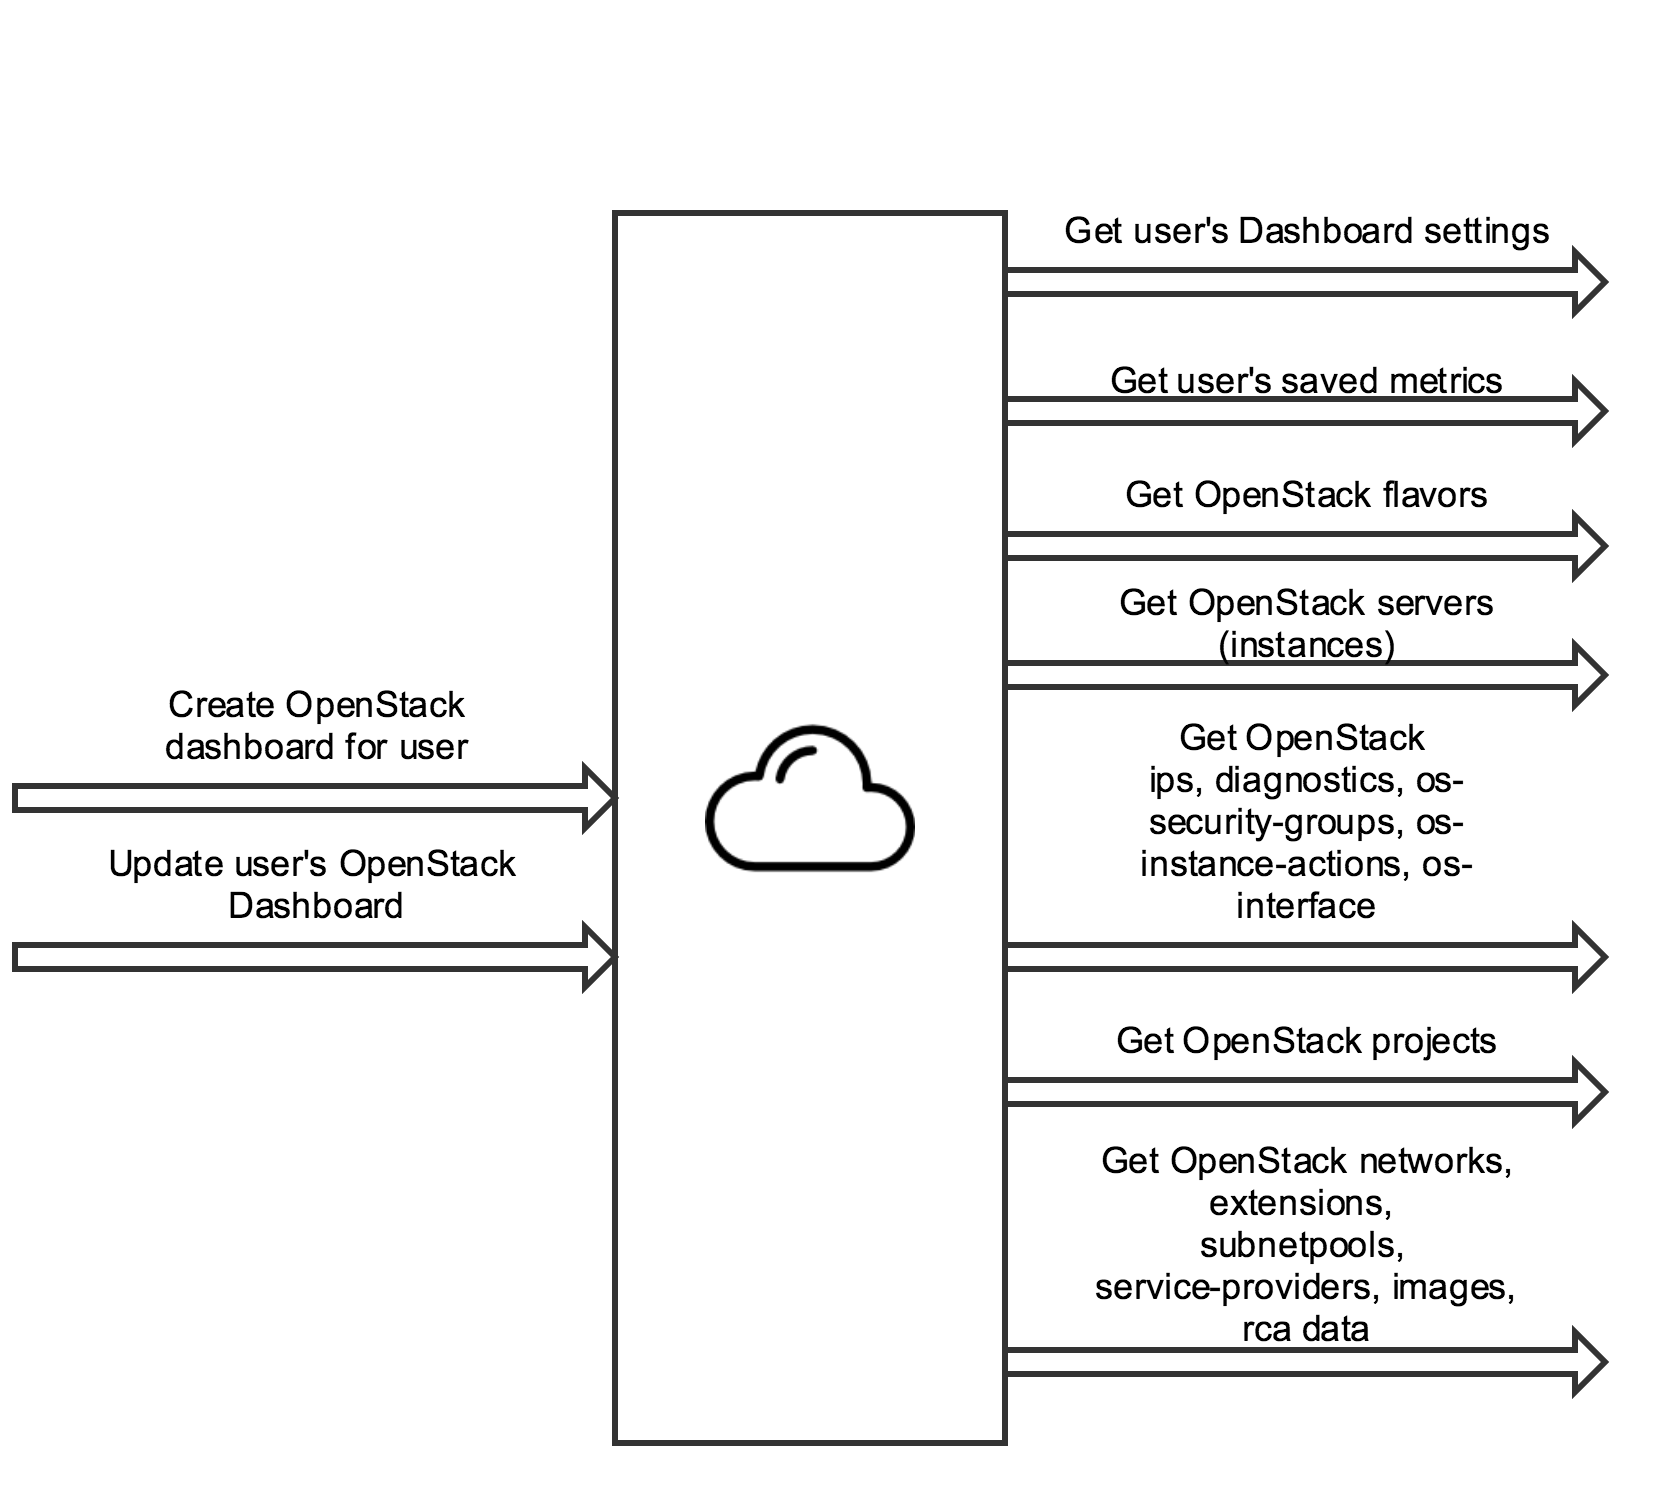
\includegraphics[width=\linewidth]{components/3/components/cloud_service.png}
  \caption{N2Sky Cloud Management Web Service}
  \label{fig:cloud_service}
\end{center}
\end{figure}

 
 As shown in figure \ref{fig:cloud_service} Cloud Management Web Service has following accessible services:

\begin{itemize}
\item Get users Dashboard settings
\item Get users saved metrics (reference to \autoref{Continuous Monitoring System} )
\item Get OpenStack Services: flavours, servers, networks, images etc.
\item Create / Update users OpenStack Dashboard settings
\end{itemize}

Detailed information about web service API and API documentation can be found in \autoref{API Documentation}


\subsection{Continuous Monitoring System}\label{Continuous Monitoring System}

In client-server architecture, especially for OpenStack cloud platform, computer servers are important. Servers could go down, but the system-administrator does not have to work 24/7 in order to monitor the system and wait until a problem occurs. A system administrator could use a monitoring tool such as Nagios for OpenStack in order to get information about each servers state. Monitoring tools can give information about the system, network, and infrastructure \cite{nagios}. The purpose of the monitoring tool is to detect issues and inform the system administrator about the occurred problem. This tool cannot solve the problem, but it can give information on what might have failed in this process.
 
\subsubsection{Monitoring Requirements}\label{Monitoring requirements}

The base monitoring system is a readable and understandable representation of the graph. Graphs allow the user to identify monitored objects and recognise their metrics. 
A good monitoring graph gives meaningful description but also helps quickly in detecting and determining issues via representation. This kind of graph should serve as a motivation while solving problems. 
Some simple rules can be followed for a precise graph representation:

\begin{description}
\item[Consistency.] Representation should correctly reflect reality. All objects, which are represented on the graph, must be correlated with a real data on the machine. 
\item[Graphs need to make sense.]  All lines represented on the chart have to be readable and understandable. Fake or unreadable information could cause problems. The metrics set should be small, one metric represent one object. There is no need to put multiple objects which do not bind directly to one chart.
\item[Stacked area vs. multiline area.] Not every chart should have the same visual representation of the lines. Depending on the case, we can decide which type of area to use. If there are small time series with high frequency, it is better to use a multiline area. A stacked area might be better on longer time series but with a bigger metric set respectively. 
\item[Understanding graph before starting to analyze it. ] Since there are going to be multiple charts with different metrics we need to make sure that every user can understand the meaning of each particular graph. Good naming, fulfilled content and correct positioning are very important.
\item[Data hierarchy. ] It is necessary to define groups, metrics, data points and nested levels on the chart.  Groups help to bind similar objects together. Data points give information of time stamps. Metrics give the actual graph representation. The nested level is a multiple line kind of metrics. All mentioned data should be visible and accessible. 
\item[Clarity.] Designing a chart is significant. There are multiple devices with different screen resolution. Too many lines on limited space will make the chart unreadable. If there are lots of charts on one page, users will be confused on what the meaning of that actually is. A good practice would be to create multiple pages with grouped charts. 
\item[Perspective.] It is important to put graphs in such perspective so that any deviation will be easily noticeable. 
\item[Appeal.] All charts are user-oriented. Today, a simple and clean appearance of the application is relevant when choosing an appropriate design when a large number of charts are available.  
\item[Control and managing.] It should be possible for any user to manipulate a graph. Either to change time series or remove metric, customization of the graph makes the whole application more attractive.
\end{description}

\subsubsection{Applying Monitoring}\label{Applying Monitoring}
To build continues monitoring system, there is a need to use a toolkit with an active ecosystem. While searching for a proper toolkit one should keep in mind some specific requirements that are going to be used in N2Sky:
\begin{itemize}
\item Proper and self-describable metric name with a key pairs.
\item Possibility to query metrics and join them in one graph.
\item Not resource-intensive.
\item Support HTTP/HTTPS protocol.
\item Collect and push time series to repository.
\item Scalable.
\end{itemize}

After researching, it was decided on the Prometheus Monitoring Toolkit \cite{alert_overview}. This tool supports all demanded requirements. One of the most interesting features is that Prometheus can be used on any UNIX environment. Prometheus will match exactly our needs since the multiple instances of OpenStack which can have different operating systems.
Originally, Prometheus was created by SoundCloud team in 2012. The core of monitoring application is the Prometheus server, which collects time series data from the moment it was executed on the environment as shown in figure \ref{fig:prometherus_arch}. All components are written in Go language and support multiple modules for monitoring different environment metrics. 
To understand the nature of Prometheus it is necessary to explain its architecture. 

\begin{figure}[htbp]
\begin{center}
  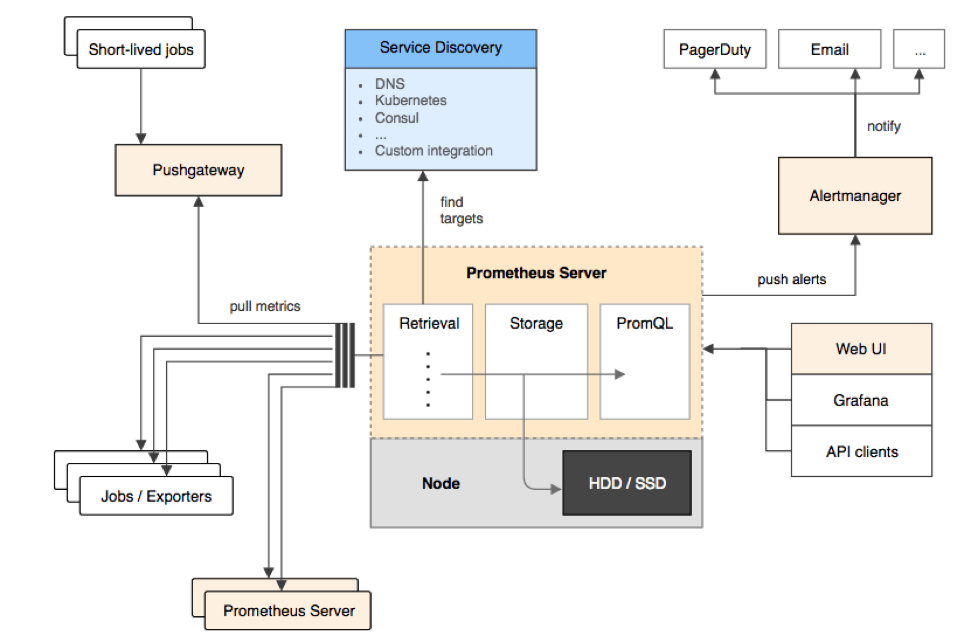
\includegraphics[width=\linewidth]{components/3/prometherus_arch.png}
  \caption{Prometheus monitoring architecture}
  \label{fig:prometherus_arch}
\end{center}
\end{figure}

The core Prometheus server pulls all metrics from jobs which are instrumented if the service is unavailable. For instrumentation, it can be pulled from gateway. All metrics and logs data is stored locally so there is no distributed storage. It is possible to query this data to retrieve more specific information about particular metrics of joint metrics. N2Sky uses Prometheus API to build own customized dashboards. 
The common components of Prometheus architecture:
\begin{description}
\item[The Prometheus server.] This is the basic element in the whole architecture. The server includes services which collect, store and retrieve nodes. The principle is scrapping or pulling. This means that the data fetched with some interval can be configured and stored accordingly as a time series. Prometheus supports different modules and each module represents a specific node. The nodes expose these ports that Prometheus uses for retrieving the data. For example, in N2Sky is being used the Node Exporter Module which gives the possibility to collect almost all essential data like CPU, RAM, HDD/SSD etc.
\item[Push gateway.] There are nodes, which are not exposing endpoints. In this case, the data collection through this Push gateway is possible. Prometheus short-lived jobs are executed to capture the data and convert it to the time series that can be used by Prometheus.
\item [Alert Manager.] Monitoring consists of multiple metrics and each metric can be analyzed. It is possible to subscribe to particular metric in order to detect metric behaviour, namely metric deviations. The Alert Management System used for firing events. It is possible to receive alert notification over multiple channels like Emails, SMS, Push notification etc.
\end{description}

Metric notation 
Following example represent metric notation:
\begin{lstlisting}
node_filesystem_avail {method="GET", endpoint="/api/posts", status="200"}
\end{lstlisting}

The metric naming is always self-described.  Requested metric "node\_filesystem\_avail" means available free space in the filesystem. Every operating system has a different metric naming. N2Sky will propose the list of available metrics. In curly brackets is defined the type of request, an endpoint and the expected HTTP response status.

After executing this query, the data will be retrieved from logs and represented as a time series as shown in figure \ref{fig:monitoring_req}.



\begin{figure}[H]
\begin{center}
  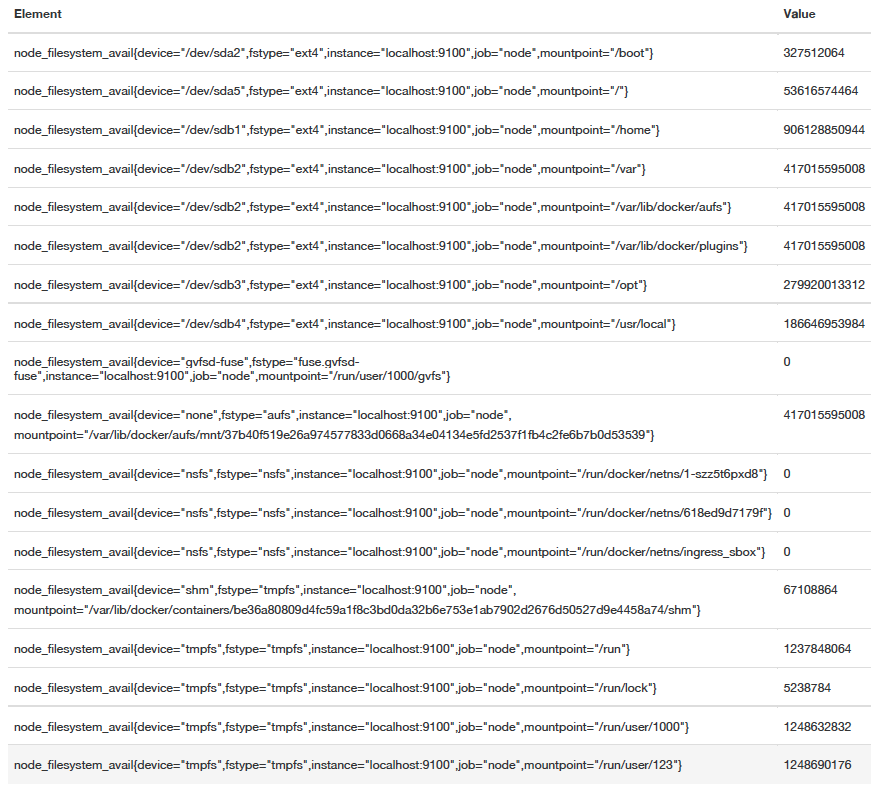
\includegraphics[width=\linewidth]{components/3/monitoring_req.png}
  \caption{Metric response}
  \label{fig:monitoring_req}
\end{center}
\end{figure}

One of the requirements of our monitoring system is scalability. One of the greatest features of Prometheus is that even if the environment is going to be overloaded, it will generate the same amount of metrics anyway. Hence the amount of events it still is independent of the amount of generated time series. 
When mentioning requirements, the possibility exists to build joint metrics, namely build multiple time series using this kind of metric:

\begin{description}
\item[Counter] The counter is a metric representing a simple numerical value which can be incremented but not inverse. One of the typical examples is a number of expectations. 
\item[Gauge] The gauge is a metric, which also represents a simple numerical value like a counter, but it is bidirectional. It means that this value can be decremented. The common example is CPU usage, which can go up and down.
\item[Histogram] The histogram is a metric, which represents observations. It is stored in a bucket, which can be pulled. Any bucket can be configured depending on the need. It can be the sum of values or count of events, which are observed.
\item[Summary] The summary is a metric, which is similar to the histogram but it calculates configurable quantities. 
\end{description}

\subsubsection{Integration with N2Sky}\label{Integration with N2Sky}

Prometheus supports query language, which is the key feature of this tool. The Prometheus query language, or promql, is expressive. 
With Prometheus, a self-described metric name can be chosen. Prometheus converts all metrics so that every human can understand what eacg particular metric means. The previous example with a metric "node\_filesystem\_avail" is a good one to show how it actually works. This metric shows the folders on root and available memory on each.

\begin{lstlisting}[caption=Prometheus query]
    node_filesystem_avail 
        {device="/dev/sdb4",fstype="ext4",
        instance="localhost:9100",job="node",
        ssmountpoint="/usr/local"}
\end{lstlisting}

Following request means that on "/usr/local" 186.6 GB is available. 

There is also the possibility to check a response code, which is especially useful for alerting. 

\begin{lstlisting}[caption=Prometheus short query]
        node_filesystem_avail {status="500"}
\end{lstlisting}

This request returns some response code 500, namely internal server error. 

For building a proper monitoring dashboard, it is important to provide customisation. Prometheus supports time duration:

\begin{itemize}
\item s - seconds
\item m - minutes
\item h - hours
\item d - days
\item w - weeks
\item y - years
\end{itemize}

Using the time duration with an offset, a user could get the exact metric on demand. 
Building query with Prometheus can bring lots of advantages. For example, there is the query which has a counter with an available node file system metric:

\begin{lstlisting}[caption=Prometheus alerting rule]
    took( 3, sum(
         rate(api_http_requests_total{status=500}[1h]
    ) )
     by (endpoint)
     )
\end{lstlisting}

This query is already complicated, but it can be extended by multiple new rules and constraints. 

In N2Sky, was developed such a monitoring service that uses the micro services approach like an entire application. It was decided to get rid of complex queries and provide some intuitive way of creating metrics. 
First of all, the time range adds complexity. It was decided that the user should give only the time interval and step. In an example when the user wants to see the CPU load for the last hour with a step 30 seconds. It makes the creation of metric more intuitive, no more range like "from", "to" and other types of ranges. All this can be solved with one simple request. 
The second part is the storing of metrics. Instead of every time building a query, the monitoring service will save the requested by user metric. In this case, every user will get his own customised metric. 
The service uses Mongo DB for storing of the metric configuration. Every collection has its own schema. When a user makes a request to save a metric, the schema has to be filled with the requested by user data.


The benefit of the microservices architecture is the independence of each service. The good part of it is that when one of the services is not be accessible, the rest of them would still be up and running. The problem is that in order to make the application running in the correct way, all services are required. It is important to detect events and rollbacks or transactions in case if an error or failure occurs. N2Sky has its own monitoring and alerting system, which notifies the system administrator about failures. The problem is how to handle events, which are transactionally dependent from service to service in case of an occurring error and how an event is handled when still in transaction. There is two main kind of events \cite{cs5366}: 

\begin{itemize}
\item \emph{Intrinsic Events.} Process steps starting and finishing generate events intrinsic to the process model. This kind of events contains the process step or failure. 
\item \emph{Context Events.} Events stemming from the context of the process.
\end{itemize}

It is impossible to maintain each event and process an event stream in the N2Sky application. If other developers forget to put the event into the stream, it will unnoticeable. That is why in N2Sky are events intrinsic, which log every transaction from one service to another. In case of an error, the alerting event will be fired with a log data which contain the step and the error itself.  


\subsubsection{Monitoring Dashlet Design}\label{Monitoring dashlet Design}

Since multiple machine and services are being monitored, there was a need to create a dedicated dashboard design. At first, the to-be-monitored environments would be: 
\begin{description}
\item[Openstack Machine.]  It is a dedicated machine, our cloud base for development and running instances.
\item[Openstack Instances.]   Virtual machines with a different OS.
\item[Docker Containers.]  Virtual machines in the OpenStack instances.
\end{description}

One of the most important parts of application design is to maximize reusability of the components. 

 
\begin{figure}[htbp]
\begin{center}
  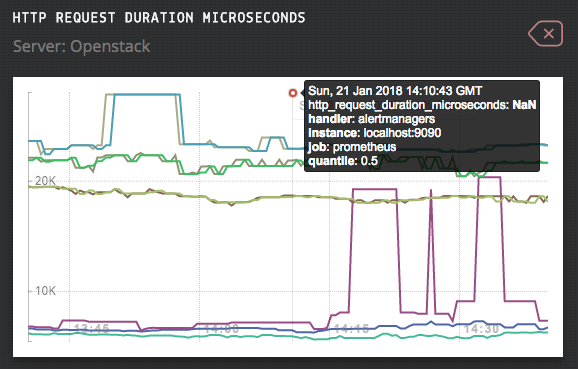
\includegraphics[scale=0.65]{components/3/components/monitoring_dashlet.png}
  \caption{N2Sky Monitoring Dashlet}
  \label{fig:monitoring_dashlet}
\end{center}
\end{figure}

 
The figure \ref{fig:monitoring_dashlet}  shows a HTTP request directions in milliseconds metrics. Each dashlet item contains:
\begin{itemize}
\item Title, which represents a readable and self-described metric name.
\item Server, which shows to which instance this metric belongs.
\item Chart, which is the monitoring data itself. 
\item Tooltip, which appears on metric mouse over. Tooltip shows following data:
\begin{itemize}
\item Date of the particular position.
\item Name of metric.
\item Instance environment.
\item Handler is an alert manager listener (reference to \autoref{Alerting Management System}).
\item Cron job.
\item Quintile.
\end{itemize}

\end{itemize}


\subsection{Alerting Management System}\label{Alerting Management System}

Today, the most trending subject in the monitoring area is a prediction and automated detection. It makes the system-administration free from 24/7 managing, maintaining, and monitoring system.
For monitoring, the Prometheus tool is the used one. Since this tool is constantly saving data logs about the system, it is possible to reuse these logs to build an alert system. 
Prometheus tool provides an Alert Manager module. Natively, this tool supports different notification methods like email notification or some request on Slack. 

\subsubsection{Alerting System Architecture}\label{Alerting System Architecture}

Since the Alert Manager is a part of Prometheus Tool, it has its own binary application. The idea behind is to have only one Alert Manager and have monitoring tools on multiple machines. If the machine goes down or even Prometheus itself, the Alert Manager can catch and deliver this event. 
To understand how the Alert Manager works, it is essential to understand the architecture of the whole system as displayed in figure \ref{fig:alert_arch}.

\begin{figure}[htbp]
\begin{center}
  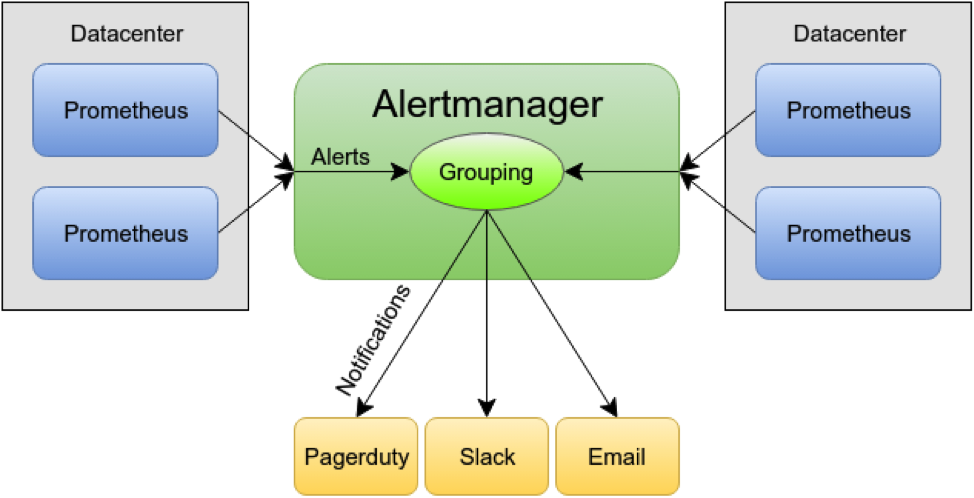
\includegraphics[scale=0.6]{components/3/alert_arch.png}
  \caption{Alerting System Architecture}
  \label{fig:alert_arch}
\end{center}
\end{figure}

This architecture is a typical messaging platform.
The Messaging Service sends messages to multiple clients. It is implemented in the Producer-Consumer Pattern. In the Alert Manager Architecture, the role of the producer is taken by Prometheus Datacenter. Alert Manager consumes the messages. The consumer knows nothing about the producer but just subscribes to the event. With this approach, multiple producers can be attached \cite{alert_book}. 

Alerts can be collected in groups by the datacenter. If an event occurs on multiple machines, it can be packed into one notification and accordingly fired . 
In the Prometheus configuration, two things should be set up: reference on Alert Manager and Alert Rules. When the Alert Manager consumes an event, it just dispatches it via notification as displayed in figure \ref{fig:alert_arch_detailed}.

\begin{figure}[H]
\begin{center}
  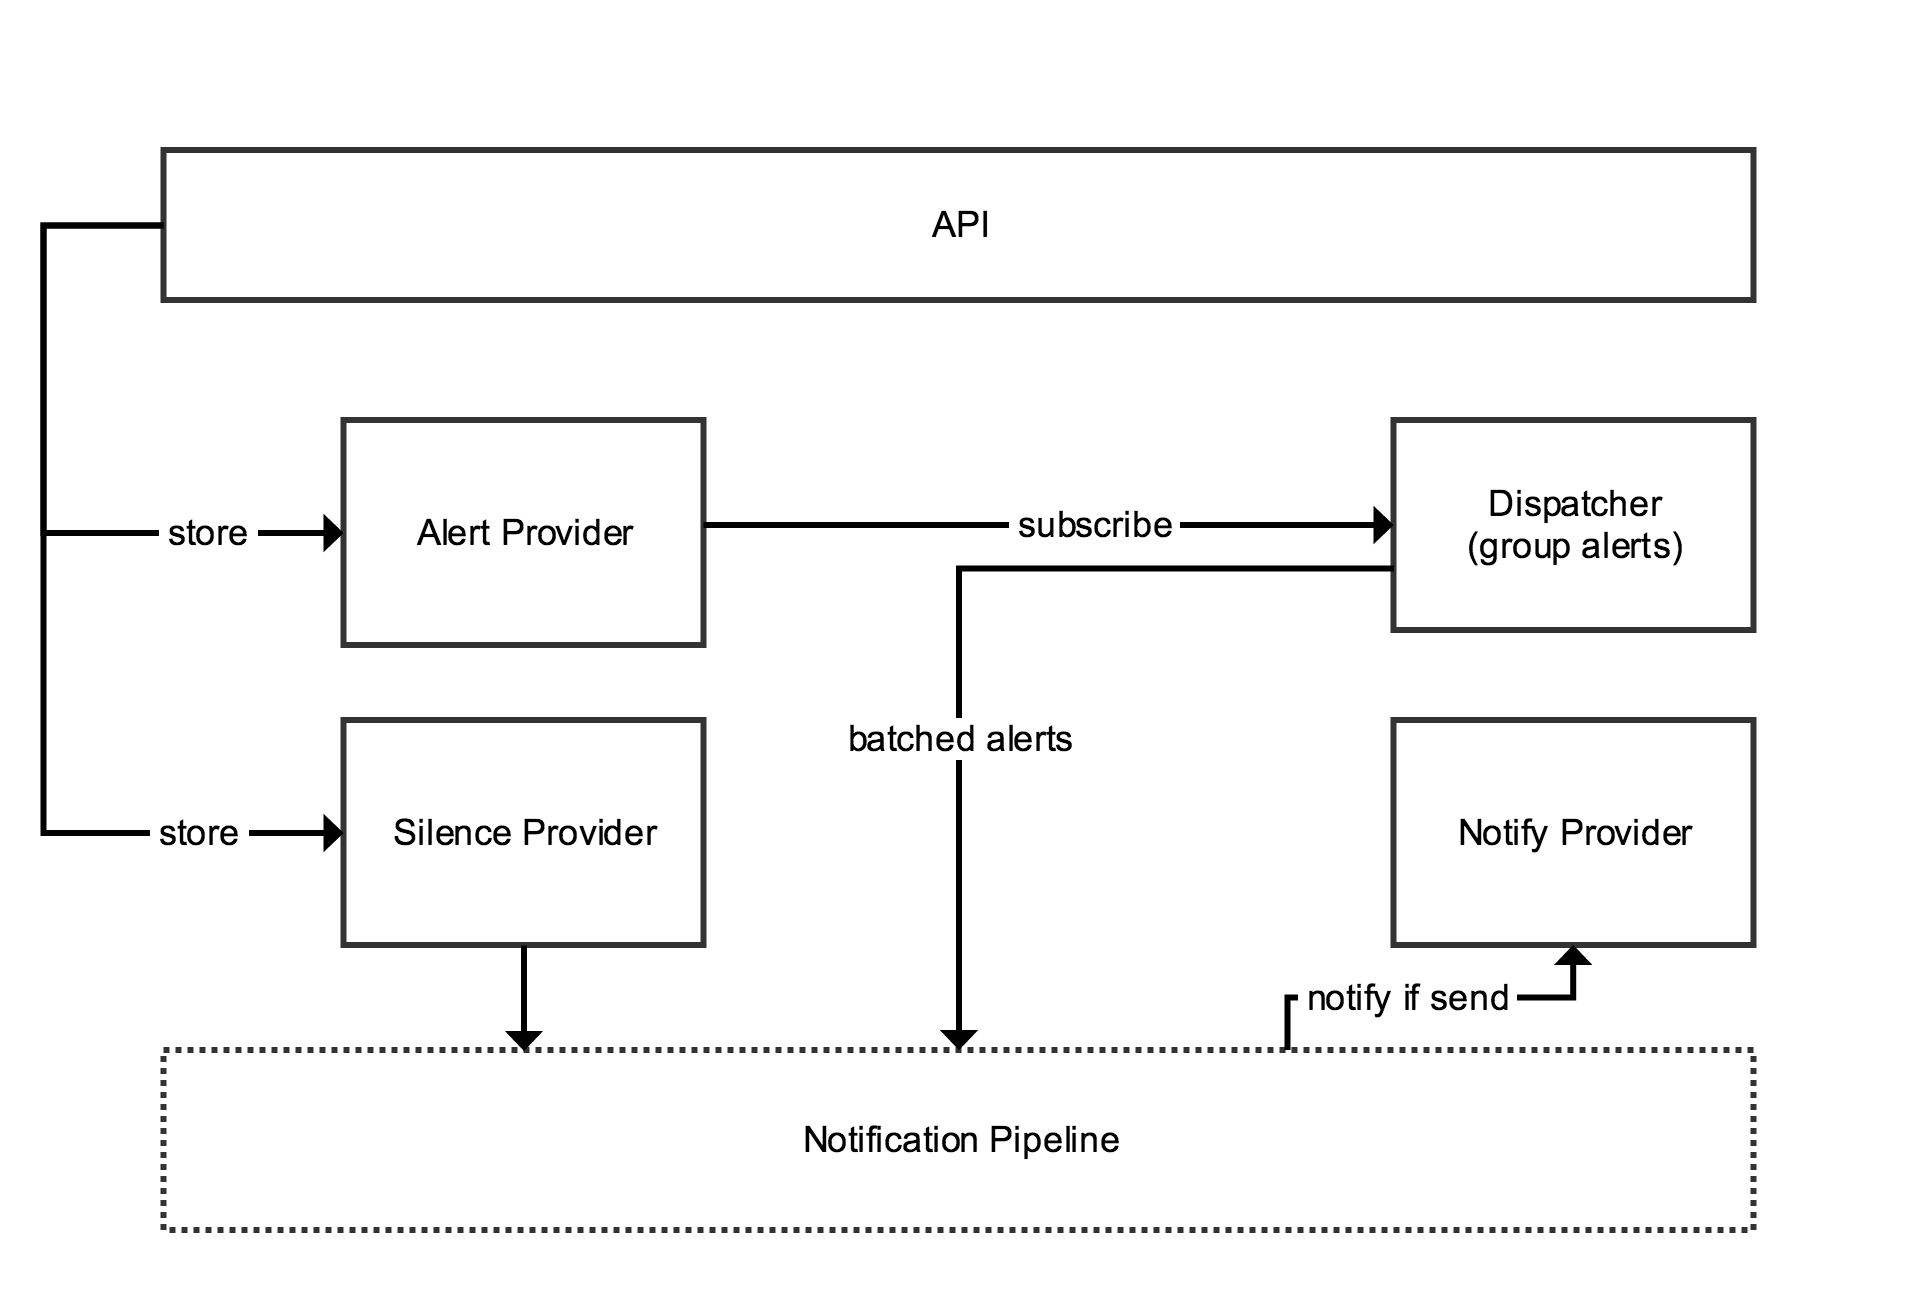
\includegraphics[width=\linewidth]{components/3/alert_details.png}
  \caption{Communication within Alerting Management System}
  \label{fig:alert_arch_detailed}
\end{center}
\end{figure}

\begin{description}
\item[API] Alert manager API has only one endpoint, which gives the list of events that occurred.
\begin{lstlisting}
            /api/v1/alerts
\end{lstlisting}

As a response the event information is sent \cite{alert_send}.
 \begin{lstlisting}[caption=Querying alert]
 [
  {
    "labels": {
      "<label>": "<value>"
    },
    "annotations": {
      "<label>": "<value>",
    },
    "startsAt": "<date>",
    "endsAt": "<date>"
    "generatorURL": "<url>"
  }
]
\end{lstlisting}
The following response shows the timestamp of the event, additional information as an annotation and name of event (alert). 
\item[Silences.] Silences are commands, which mute alerts for specific time. It can be configured via web interface. 
\item[Dispatcher.] The Dispatcher is a grouping of alerts with a similar nature into a single notification. This will be send as a batch to Notification pipeline.
\item[Notification Pipeline.] A pipeline which consists on channels, routers and filters. It takes rules from Alert Provider and Silence Provider and alerts from Dispatcher. If a notification is ready, it can be send. 
\end{description}


\subsubsection{Alert Rules}\label{Alert Rules}

As it was mentioned, one of the main changes in the Prometheus setup, is to configure the alert rules. Every Prometheus Monitoring Tool can have its own alerting rules, which can be defined. There is also a possibility to reference on common alerting rules for every monitoring system on every machine. 

 \begin{lstlisting}[caption=Alert error response]
        groups:
        - name: test
          rules:
          - alert: Error
            expr: job:request_latency_seconds:mean5m
            {job="loclhost:5000"} > 0.5
            for: 5m
            labels:
              severity: page
            annotations:
              summary: latency
\end{lstlisting}

The following example of alerting rules shows the typical alerting rule. The most important part is an expression, which is applied to the Monitoring System. More details about the creation of alerting rules are located in the Development Guide chapter "Setting up Alert Management System" \autoref{Setting up Alert Management System}.

Alerting rules are instructions to the monitoring system and can be useful for alerting as well as for recording. 

Recording rules allow to pre-compute frequently needed expressions or expressions, which are resource or time-consuming.  These rules are saving the result in a new set of time series. It is like indexing this data, so that prevent expansive I/O methods. 
The rules are being executed sequentially with a predefined interval. 
With an alerting rule, it is possible to define an alert, i.e deviation by particular expression from the Prometheus Tool and its exports (modules). It allows the building of an alert even on the combined query. 

In case that the Alert Manager is not available, all alerts are saved into the buffer. As soon as the Alert Manager will be online, all events will be fired sequentially. 



\subsubsection{Integration with N2Sky}\label{Integration with N2Sky Alerting}

The Alerting System is represented as a module in N2Sky. 
Alerting Client is the additional configuration of Prometheus Monitoring System. When Prometheus will be executed, it should have the reference to Alerting System and its rules. 
Since the client should be installed on each OpenStack instance, it was integrated into the image snapshot. When the new instance will be spawned with an OpenStack snapshot, the client will be automatically executed there.  

Alerting Client fire alerts depend on configured rules. The rules can be created via the user interface. The list of events N2Sky receives via its service it is fetched information from the Alert System. 
 
\subsubsection{Alerting System Design}\label{Alerting System Design}

Alerting System UI kept the same design as in the entire application. The N2Sky UI components were reused and no new component was created. The main component is a grid item which contains information about an event, which occurs as shown in figure \ref{fig:alert_grid}.

\begin{figure}[htbp]
\begin{center}
  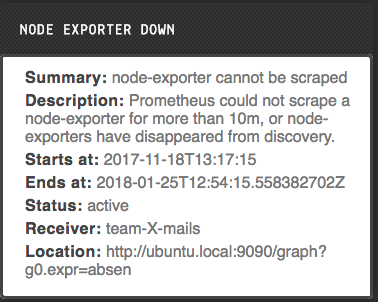
\includegraphics[scale=0.7]{components/3/alerts/alert_grid.png}
  \caption{N2Sky Alerting Management System Event representation.}
  \label{fig:alert_grid}
\end{center}
\end{figure}

The following information is shown:

\begin{description}
\item[Title.] The name of alert.
\item[Summary.]  It is a short description of the alert. If the summary is too long, it will be cut.
\item[Description.] The whole description of the alert.
\item[Starts at.] Timestamp when the event occurred. 
\item[Ends at.] Timestamp when the event is no more valid. If the timestamp is a current day and time, the problem is not yet fixed. 
\item[Status.] Actual status of the event. Can be active and inactive.
\item[Receiver.] The group of receivers. Normally, the group contains multiple receivers emails. 
\item[Location.] The endpoint of the server where the monitoring system is installed. 
\end{description}

Every alert has its severity level. Depending on it, the fired events will be represented differently. Every severity level has its own color on N2Sky as shown in ``Fig.~\ref{fig:alert_severity}''.

\begin{figure}[htbp]
\begin{center}
  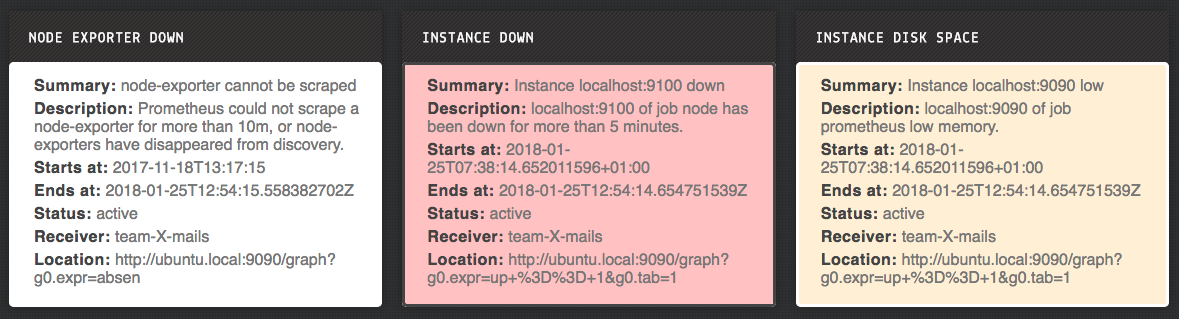
\includegraphics[width=\linewidth]{components/3/alerts/alert_severity.png}
  \caption{N2Sky Alerting Management System Severity Level}
  \label{fig:alert_severity}
\end{center}
\end{figure}

There are three types of severity levels:
\begin{itemize}
\item Critical, which shows that a crucial event occurs. For example, if the server goes down, it is a critical severity level.  In N2Sky, the UI is red. 
\item Warning, which shows that something went wrong. For example, not enough disk space on the server. In N2Sky, the UI is orange. 
\item Page, which shows information. For example, lots of requests occurred. In N2Sky, this UI is white.  
\end{itemize}
 



